{\Huge \bfseries \noindent Chapter 5}
\vspace{-1em} 
\section*{\LARGE Competing endogenous RNA axis defines a prognostic signature for biochemical recurrence in prostate cancer}
\addcontentsline{toc}{section}{5\quad Competing endogenous RNA axis defines a prognostic signature for biochemical recurrence in prostate cancer}
\setcounter{section}{5}
\setcounter{subsection}{0}  % reset so next \subsection is 2.1
\renewcommand{\chapternum}{5}

% Reset figure/table numbering after chapter 4 supplementary overrides
\renewcommand{\thefigure}{\chapternum.\arabic{figure}}
\setcounter{figure}{0}
\renewcommand{\thetable}{\chapternum.\arabic{table}}
\setcounter{table}{0}


\begin{center}
    \textit{The contents of this chapter are currently under peer review at Scientific Reports}
\end{center}


\subsection*{Abstract}
Androgen deprivation therapy is the mainstay for the treatment of localised prostate cancer, yet one in three patients progress towards a castrate-resistant prostate cancer phenotype. Second-generation anti-androgen drugs such as enzalutamide show overall benefits to survival in castrate-resistant prostate cancer patients; however, patients ultimately acquire resistance to enzalutamide, progressing to metastatic castrate-resistant prostate cancer. In this study, we constructed a circular RNA–micro RNA–messengerRNA competing endogenous RNA network by integrating transcriptomic profiles from enzalutamide-resistant LNCaP cell lines and prostate cancer patients experiencing biochemical recurrence. Messenger RNAs within this shared regulatory network were used to derive a prognostic gene signature across nine independent prostate cancer cohorts with time-to-biochemical recurrence metadata. Model robustness and generalisability were assessed using internal–external cross-validation, bootstrap resampling, validation in an independent external dataset and comparisons to published signatures. We present a 23-gene prognostic signature that predicts biochemical recurrence within five years and is largely distinct from previously published signatures, highlighting the utility of modelling transcriptomic signatures through the lens of regulatory RNA interactions.




\subsection{Introduction}\label{sec1}
Prostate Cancer (PCa) is the second most frequently occurring cancer and the fifth leading cause of cancer-associated deaths in men \cite{Sung2021}. Radical prostatectomy, external beam radiotherapy or brachytherapy are the mainstay of treatment for localised PCa. Approximately 35\% of men experience biochemical recurrence (BCR) after treatments defined by three consecutive rises in prostate-specific antigen (PSA) levels 1 week apart \cite{Rans2022}, progressing to castrate-resistant prostate cancer (CRPC), increasing the risk of distant metastasis and poor survival outcome \cite{Shore2024}. Enzalutamide is a second-generation androgen deprivation therapy drug administered to patients experiencing postoperative recurrence events, competitively binding the androgen receptor (AR), impeding AR signalling and arresting PCa growth \cite{Koochekpour2010}. Despite overall survival benefits of 4.8 months in patients, between 20\%-40\% are intrinsically resistant, whilst all patients will eventually acquire resistance to the drug as measured by increasing PSA levels \cite{Scher2012Sep, Cornford2017}. There is therefore an increasing need to identify biomarkers associated with biochemical recurrence to guide treatment options for PCa patients, improving quality of life and overall survival.

Next-generation sequencing (NGS) provides researchers with a powerful tool to detect biomarkers in clinical samples. The preparation times, sequencing time, and costs associated with NGS technologies are consistently reducing, making NGS a cost-effective tool for biomarker discovery \cite{Lopez2015}. RNA biomarkers are of particular interest, as they provide a snapshot of dynamic cellular states compared to DNA biomarkers and also exhibit superior sensitivity and specificity compared to protein biomarkers \cite{Nimse2016, Xi2017}. The ENCODE project revealed that 76\% of the human genome is transcribed, but only 1.2\% of this represents protein-coding genes \cite{Consortium2012, Djebali2012}, resulting in an increased interest in non-coding RNAs (ncRNAs) and their role in gene regulation. 

Non-coding RNAs (ncRNAs) can be categorised as small ncRNAs ($\le$200nt length) comprising micro RNAs (miRNAs), piwi-interacting RNAs (piRNAs), small nucleolar RNAs (snoRNAs), and long non-coding RNAs (lncRNAs) ($\geq$200nt length). More recently, circular RNAs (circRNAs), originally believed to be aberrant by-products of splicing \cite{Cocquerelle1993Jan, Qian1992}, have emerged as a class of ncRNAs. circRNAs harbour functionally active and evolutionarily conserved miRNA response elements (MRE) within their mature spliced sequence, which are capable of sequestering miRNAs and have been shown to act as competitive endogenous RNAs (ceRNAs) in circRNA-miRNA-mRNA regulatory networks \cite{Thomas2014Aug, Hansen2013Mar, Denzler2014Jun}. Several studies detailing the role of ncRNAs in PCa have since emerged, identifying potential molecular biomarkers and new therapeutic strategies advancing our understanding of disease progression \cite{Aird2018, Bolton2014, Ghiam2017, Ding2021, Takayama2015}.

Recently, several studies have sought to identify prognostic markers by exploring the ceRNA network in diseases \cite{He2022Dec, Song2020Aug, Huang2023Oct, Zhang2023Dec, Guo2020Jul, Shang2025May}. This strategy reduces the input feature space for prognostic modeling by performing differential expression analysis at three levels (circRNA, miRNA, and mRNA), predicting RNA–RNA interactions, and filtering by direction of fold change to construct tri-partite circRNA–miRNA–mRNA graphs that reflect predicted ceRNA network activity. In contrast, traditional approaches that rely on differential expression analysis, dimension reduction, supervised machine learning, or any combination thereof solely at the gene level, may overlook regulatory interactions between RNA biotypes.

Whilst such studies are novel in the sense of incorporating regulatory networks, they are not immune to the common pitfalls of reporting model transparency \cite{Dhiman2021Oct}. Authors typically report the prognostic model's validation in the training dataset and external validation results, which can be severely overoptimistic in studies lacking appropriate power due to overfitting \cite{Steyerberg2015Apr}. Furthermore, authors may neglect to report heterogeneity in model performance across relevant patient groups, thereby omitting information regarding model generalizability \cite{Riley2016Jun}.

In this study, we develop a prognostic model capable of predicting BCR and validate our prognostic model through internal-external cross-validation, bootstrap resampling, optimism-corrected apparent performance, and external validation to ensure transparency in model performance. The code used to perform the analysis is available at \href{https://github.com/BarryDigby/pca_network}{BarryDigby/pca\_network}, facilitating reuse and adaptation to future research.


\subsection{Methods}\label{sec2}

\subsubsection{Data collection}\label{methods1}
Differential expression analysis and subsequent ceRNA network construction were performed using two circRNA datasets, seven miRNA datasets, and five mRNA datasets (Supplementary Table \ref{chp4supptable1}, Supplementary Table \ref{chp4supptable2}, Supplementary File \hyperlink{chp4suppfile1}{1}). Each RNA biotype group included at least one dataset comparing primary PCa to normal tissue, and at least one dataset comparing enzalutamide-resistant to enzalutamide-sensitive samples. Prognostic model development and validation were performed using ten survival PCa datasets containing time to BCR, Gleason score and PSA level metadata (Supplementary Table \ref{chp4supptable3}).

\subsubsection{Data processing}\label{methods2}
Quantile normalized, log2 transformed circRNA, miRNA and mRNA microarray datasets (GSE113153, GSE118959, GSE45604, GSE46738, GSE143408 and GSE78201) were downloaded using GEOquery \cite{Davis2007} and analysed in R (version 4.2.0). GSE21036, GSE23022 and GSE36803 miRNA and mRNA raw CEL files were downloaded from ArrayExpress \cite{Parkinson2007}, RMA normalised, and Log2 transformed using the oligo package \cite{Carvalho2010} prior to differential expression analysis. GSE88752, TCGA-PRAD miRNA and TCGA-PRAD mRNA count data were normalised with respect to library size using edgeR \cite{Robinson2010Jan} and transformed using limma-voom \cite{Law2014Feb}. 

In-house LNCaP small RNA-Sequencing data were processed using custom scripts available on GitHub. Briefly, the reference miRBase hairpin FASTA file was downloaded and converted to DNA sequences using \textit{seqkit seq --rna2dna} before indexing using Bowtie \cite{Bowtie, Shen2016}. Next, raw sequencing reads were subject to adapter removal using the TruSeq smallRNA adapter sequence, clipping 4 bases from the 5' and 3' ends of reads and filtering to remove reads of length $<$17nt or $>$30nt \cite{Krueger2023}. The processed reads were collapsed using \textit{seqcluster collapse} and aligned to the reference hairpin file using Bowtie \cite{Pantano2016, Bowtie}. For each read, 2 mismatches were allowed in the seed region, and the optimal alignment was selected from the 50 reported alignments using \textit{-n 2 -k 50 --best --strata}. Candidate miRNAs were quantified against the miRBase GFF file using \textit{mirtop} with default parameters \cite{Desvignes2020}. In-house LNCaP RNA-Sequencing samples were processed using the `STAR-Salmon' transcript quantification subworkflow in nf-core/rnaseq v3.12.0 \cite{Patel2023}. 

Pre-normalised log2 CPM RDS files were downloaded from PCaDB and used for prognostic model development \cite{Li2022Jan}. Each dataset was centred and scaled, with duplicate gene identifiers collapsed to select the highest variance.

\subsubsection{Identification of co-expressed differentially expressed RNAs}\label{methods3}
Limma \cite{Ritchie2015} was used to identify differentially expressed circRNAs, miRNAs and mRNAs in each respective dataset, with an adjusted \textit{P} value $\leq$0.05 after Benjamini-Hochberg multiple testing correction deemed statistically significant. Co-expressed circRNAs, miRNAs and mRNAs were identified by selecting probes/genes that are present in both PCa vs. normal and enzalutamide-resistant vs. enzalutamide-sensitive limma TopTable results, and exhibit the same fold change direction. Custom scripts were used to convert both Arraystar human circRNA microarray V2 probes to circbase IDs and outdated miRNA probe IDs to their latest miRBase aliases, ensuring standardisation of results and compatibility with downstream target prediction analysis.

\subsubsection{circRNA, miRNA, mRNA target prediction}\label{methods4}
The predicted miRNA targets of screened differentially expressed (DE) circRNAs were obtained using the CircBase database \cite{circbase} and the Cancer-Specific CircRNA Database \cite{CSCD}, generating database-guided circRNA-miRNA pairs. DE-miRNAs were subsetted using the intersection of the predicted circRNA-miRNA targets. Finally, the gene targets of DE-miRNAs were obtained using miRBase \cite{mirbase}, miRTarBase \cite{mirtarbase}, miRNet \cite{mirnet}, and TargetScan \cite{Targetscan}. Predicted miRNA-mRNA targets were intersected with DE-mRNAs to produce a DE-circRNA/DE-miRNA/DE-mRNA tripartite graph of predicted interactions.

\subsubsection{Construction of ceRNA network}\label{methods5}
In addition to identifying circRNA-miRNA and miRNA-mRNA pairs via sequence-specific context, the expression profiles of each pair were incorporated to deduce the final ceRNA network by selecting pairs with opposite fold change direction. The resulting circRNA-miRNA-mRNA tripartite graphs passing filtering exhibited downregulated-upregulated-downregulated and upregulated-downregulated-upregulated expression patterns, respectively.

\subsubsection{Prognostic model development}\label{methods6}
Prognostic model development using DE-mRNAs in the ceRNA network in addition to the clinical covariates Gleason score and PSA, was carried out using a dataset comprising the Belfast, CIT, CMap, CPC, DKFZ, GSE54460, Stockholm, TCGA, and Taylor datasets—henceforth referred to as the derivation dataset. The CoxBoost algorithm was chosen for feature selection with parameters \textit{minstepno} and \textit{maxstepno} set to 5 and 35, respectively, to generate a model with \textit{n} predictors that would satisfy the number of events per predictor ranging from 15-50 \cite{Harrellbook, Ogundimu2016Aug, Wynants2015Dec, Austin2014Nov}. The coefficients of the final model were extracted and used in a multivariate Cox proportional hazards model to assess the Schoenfeld residuals \cite{Schoenfeld1982}; predictors violating the assumptions were removed from the final prognostic model. 

\subsubsection{Prognostic model evaluation}\label{methods7}
\paragraph{Performance in derivation and external validation dataset}\label{methods71}
The discriminative power, overall model fit and predictive accuracy of the prognostic model in the derivation and validation datasets were calculated as detailed in Royston et. al \cite{Royston2013}: 1) The calibration slope in the validation dataset was computed and compared to the slope of the derivation dataset. A calibration slope $<$1 suggests less discriminative power, whilst a slope $>$1 indicates superior discriminative power in the validation dataset. 2) The overall fit of the prognostic model in the validation dataset was computed via a joint test of all predictors whilst constraining the prognostic index to 1. A small Chi-squared test value and a non-significant \textit{P} value indicate a good fit of the prognostic index in the validation dataset. 3) Harrell's C-index was computed for both the derivation and validation datasets; agreement between the two datasets being indicative of similar predictive performance. 4) Kaplan-Meier survival curves between risk group strata, as defined by the median prognostic index value, were plotted in conjunction with the log-rank \textit{P} value to provide empirical evidence of discrimination. 5) Hazard ratios for the high-risk groups were computed in the validation and derivation datasets. Ideally, the hazard ratio in the derivation dataset should be well maintained in the validation dataset and remain statistically significant. 6) ROC analysis revealed the overall predictive accuracy of the model via AUC. 

\paragraph{Optimism-corrected performance using bootstrap}\label{methods72}
Model optimism was estimated following the procedure described by Harrell et al. \cite{Harrell1996Feb}. 1) A model was fitted to the full derivation dataset to calculate the apparent discrimination $(c_{\text{app}})$. 2) Two hundred bootstrap samples ($M=200$) were generated using resampling with replacement from the derivation dataset. 3) For each bootstrap sample $(m=1, \ldots, M)$, predictor selection and model fitting were performed using the same approach as in step 1 to generate a bootstrap model. The model was then applied to its corresponding bootstrap sample to calculate discrimination $(c_{\text{boot}}^{\phantom{(}}(m))$. 4) For each bootstrap model, discrimination on the original derivation dataset $(c_{\text{orig}}^{\phantom{(}}(m))$ was also calculated. Coefficients from step 3 were fixed to estimate the degree of overfitting due to variable selection. 5) For each iteration, model optimism was calculated as $o^{\phantom{(}}(m) = c_{\text{orig}}^{\phantom{(}}(m) - c_{\text{boot}}^{\phantom{(}}(m)$. The average optimism across all bootstrap samples was computed to obtain the overall optimism of the original model. 6) Finally, the optimism-corrected performance of the model was reported as $c_{\text{adj}} = c_{\text{app}} - o$, providing an estimate of the expected discrimination in external validation.


\paragraph{Internal-external cross-validation}\label{methods8}
To further assess the generalizability of our model, we conducted internal-external cross-validation across the nine studies in the derivation dataset. In each iteration, one study was held out as an independent validation set, while the model was trained using the remaining studies. Importantly, the model coefficients were fixed after training on each combination of development studies and were then directly applied to the held-out dataset, without any refitting or recalibration. This ensures that performance metrics reflect true external validation, avoiding optimistic bias from adapting the model to each test set. Model discrimination was evaluated in each dataset using the steps described in section \ref{methods71}. Calibration slope and Harrell's C-index metrics were pooled across all folds using random-effects meta-analysis to provide an overall summary of performance and an estimate of model heterogeneity.

\paragraph{Comparison to published signatures}\label{methods9}
30 published PCa prognostic signatures (Supplementary Table \ref{chp4supptable4}) were collected and used to create multivariate Cox proportional hazards models representative of each signature. Each signature's performance was assessed as described in section \ref{methods71} using the external validation dataset and compared to our prognostic model derived using a ceRNA network. Coefficients for the published PCa signatures were largely unavailable; thus, comparisons between each model is based on feature selection alone and does not include analysis of coefficient estimation. Notably, the published signatures did not include any clinical covariates.


\subsection{Results}
\subsubsection{Identification of ceRNA network}\label{results1}
The contrasts used in the DE analysis of each RNA dataset and the summary of their results are provided in Table \ref{table1}. Differential circRNA expression analysis revealed 232 DE-circRNAs (168 up-regulated, 64 down-regulated). Target prediction of DE-circRNAs was performed using the CircBase and CSCD databases, returning 30,727 predicted circRNA-miRNA pairs. The intersection of the 30,727 predicted circRNA-miRNA interactions with 42 DE-miRNAs (16 up-regulated, 26 down-regulated) yielded a final set of 42 DE-miRNAs. TargetScan, miRNet, miRTarBase, and miRBase returned 61,193 miRNA-mRNA target predictions based on the 42 input DE-miRNAs. Predictions were intersected using 1,310 DE-mRNAs returned by differential gene expression analysis (691 up-regulated, 619 down-regulated), resulting in a set of 1,090 DE-mRNAs. The preliminary ceRNA network consisting of 232 circRNAs, 42 miRNAs, and 1,090 mRNAs was filtered based on the ceRNA hypothesis --- circRNA-miRNA and miRNA-mRNA pairs were filtered to include pairs exhibiting inverse expression as determined by log fold change sign --- to generate a ceRNA network consisting of 124 circRNAs, 38 miRNAs, and 817 mRNAs. The ceRNA network, including logFC values, is available in the Supplementary\_3.csv file.


\subsubsection{Prognostic model development}
The 817 DE-mRNAs identified in the ceRNA network were used to derive a model predictive of BCR in PCa. 679 DE-mRNAs were present in the derivation dataset, which in combination with the clinical covariates Gleason score and PSA, resulted in 681 predictors used as input to the Coxboost algorithm. 26 non-zero coefficients were returned by the model, with 3 predictors removed for violating proportional hazards assumptions. The 23-gene signature is presented with exponentiated coefficients, confidence intervals and \textit{P} values in Figure \ref{Figure1}A. \par


\begin{table*}[ht!]
\caption[Differentially expressed RNA biotypes]{\textbf{Differentially expressed RNA biotypes} returned by Limma and unique overlapping RNAs with the same fold change direction.\label{table1}}

\begin{adjustwidth}{-0.0in}{-0.0in}
\tabcolsep=0pt%%
\footnotesize
\resizebox{\textwidth}{!}{
\begin{tabular*}{\textwidth}{@{\extracolsep{\fill}}lllrr@{\extracolsep{\fill}}}
\toprule
\textbf{Data type} & \textbf{Series} & \textbf{Contrast} & \textbf{DE-up} & \textbf{DE-down} \\
\midrule
  circRNA & GSE113153 & Gleason high vs. low & 2,608 & 1,979
  \\
  circRNA & GSE118959 & Clone 1 vs. control & 591 & 729 
  \\ 
  circRNA & GSE118959 & Clone 9 vs. control & 20 & 74
  \\ 
  \midrule
  & & Unique overlapping circRNAs: & 168 & 64
  \\
  \midrule
  miRNA & GSE21036 & Tumor vs. normal & 153 & 145
  \\ 
  miRNA & GSE23022 & Tumor vs. normal & 17 & 8 
  \\ 
  miRNA & GSE36803 & Tumor vs. normal & 36 & 92
  \\ 
  miRNA & GSE45604 & Tumor vs. normal & 22 & 67 
  \\
  miRNA & GSE46738 & Tumor vs. normal & 68 & 68
  \\
  miRNA & GSE312115 & Clone 1 vs. control & 146 & 110 
  \\ 
  miRNA & GSE312115 & Clone 9 vs. control & 4 & 1
  \\
  miRNA & TCGA-PRAD & Tumor vs. normal & 130 & 128
  \\
  \midrule
  & & Unique overlapping miRNAs: & 16 & 26
  \\
  \midrule 
  mRNA & GSE143408 & 7 days ENZ treated vs. 0 days & 3,829 & 3,458
  \\
  mRNA & GSE143408 & 14 days ENZ treated vs. 0 days & 5,693 & 4,792
  \\
  mRNA & GSE143408 & 21 days ENZ treated vs. 0 days & 6,128 & 4,977
  \\
  mRNA & GSE78201 & 6 months ENZ treated vs. control & 518 & 571
  \\
  mRNA & GSE88752 & ENZ-resistant vs. ENZ-sensitive & 3,564 & 2,942
  \\
  mRNA & LNCaP & Clone 1 vs. control & 4,686 & 4,379 
  \\
  mRNA & LNCaP & Clone 9 vs. control & 1,420 & 1,303
  \\
  mRNA & TCGA-PRAD & Tumor vs. normal & 3,860 & 4,506 
  \\
  \midrule
  & & Unique overlapping mRNAs: & 691 & 619 
  \\
\bottomrule
\end{tabular*}}
\end{adjustwidth}
\begin{tablenotes}%
\item[] DE: Differential Expression. Clone 1: Highly enzalutamide-resistant LNCaP cell lines. Clone 9: Moderately enzalutamide-resistant LNCaP cell lines. ENZ: enzalutamide
\end{tablenotes}
\end{table*}


\subsubsection{Evaluation of the prognostic model}
\paragraph{Derivation dataset}
Model performance in the derivation dataset demonstrated good prognostic value. The prognostic index stratified patients into high- and low-risk groups, showing clear and significant separation in Kaplan–Meier survival curves (log-rank test \textit{P} $<$ 0.0001; Figure \ref{Figure1}B). Cox proportional hazards regression analysis was performed to assess the effect size of the high-risk group, revealing a significant association with BCR outcome (HR = 1.385, 95\% CI = 1.15–1.62, \textit{P} = 4.29e-31; Table \ref{table2}). Time-dependent ROC analysis at 1, 3, and 5 years showed consistent AUCs of 0.75, reflecting stable discriminatory performance (Figure \ref{Figure1}C). Furthermore, a Harrell’s C-index of 0.73 in the derivation dataset indicates reasonable discriminative ability for predicting time to BCR (Table \ref{table2}). 

Calibration curve analysis at 1, 3, and 5 years (Supplementary Figure \ref{chp4suppfigure1}) revealed systematic deviations between predicted and observed risk. Across all time horizons, calibration curves lie below the optimal line for lower predicted probabilities, indicating initial overestimation of absolute risk before crossing above the optimal line at higher predicted probabilities, reflecting underestimation in higher-risk patients.


\paragraph{Bootstrap validation}
To assess the stability of genes in our prognostic model, we examined the frequency with which each gene was selected using the CoxBoost algorithm across 200 bootstrap samples using resampling with replacement in the derivation dataset. The top-ranking genes included RNASEH2C (105), SSTR1 (102), and SPARC (94), indicating consistent inclusion across resampled datasets. Several other genes such as BGN (84), LIX1 (68), and NEU3 (60) were also frequently selected. In contrast, features like MAPK8IP2 (21) and B4GALT1 (16) were less stable. These results highlight a core subset of genes with robust selection frequencies, supporting their potential relevance to the prognostic signal. Notably, Gleason score was the most frequently selected feature during bootstrap sampling (118), yet it was not retained during model development on the original derivation dataset. A full table of gene frequencies over the 200 bootstrap iterations is available in Supplementary Table \ref{chp4supptable5}. 
\par
Next, we assessed model performance using the optimism-corrected Harrell’s C index as described in section \ref{methods71} to account for potential overfitting. Averaging $o^{\phantom{(}}(m) = c_{\text{orig}}^{\phantom{(}}(m) - c_{\text{boot}}^{\phantom{(}}(m)$ across all bootstrap samples yielded a mean optimism of 0.04725. Subtracting this optimism from the model’s apparent Harrell’s C index of 0.7291 on the full derivation dataset produced an optimism-corrected Harrell’s C index of 0.6818. This adjusted value provides a more realistic estimate of the model’s predictive discrimination when applied to new, unseen data.

\paragraph{Internal-external cross-validation}
Overall, the prognostic model was sensitive to the effects of heterogeneity between studies in the derivation dataset. The calibration slope for external validation using the Belfast dataset was 2.28, and as low as 1.19 in the CMap dataset (Figure \ref{Figure2}). This is reflected in the calibration slope pooled estimate confidence intervals (1.61, 95\% CI=1.35-1.86). Furthermore, an $I^2$ value of 43.3\% indicates moderate heterogeneity, suggesting that a proportion of the variability in calibration slopes is attributable to differences between studies rather than sampling error.

\par

Although Harrell's C-index values varied across validation datasets (range: 0.68–0.84), the random-effects meta-analysis yielded an $I^2$ of 0.0\%, $\tau^2 = 0$, and \textit{P} = 0.89, indicating no statistical significance in between-study heterogeneity. This likely reflects the wide confidence intervals and limited number of studies, which reduces the power to detect true differences. As such, visual and numerical differences in discrimination performance across studies should still be considered when assessing model transportability. The full table displaying summary statistics for internal-external cross-validation is available in Supplementary Table \ref{chp4supptable6}.

\par

To further explore heterogeneity at the predictor level, gene-specific random slope variances were estimated using mixed-effects Cox models incorporating study as a random effect \cite{Therneau2024Aug}. The majority of genes demonstrated low variance in effect estimates across studies, indicating stable prognostic associations (Supplementary Table \ref{chp4supptable7}). However, a subset of genes exhibited moderate to high random slope variances, highlighting potential heterogeneity in their effect sizes between cohorts. For example, genes PHYHD1, LIX1, MTERF4, and SPARC showed elevated variance estimates (up to 0.13), suggesting variable influence on outcome depending on study context. Overall, 18 of 23 genes exhibit low variance, indicating the model can be generalised to unseen datasets. 


\begin{figure*}[!t]%
\centering
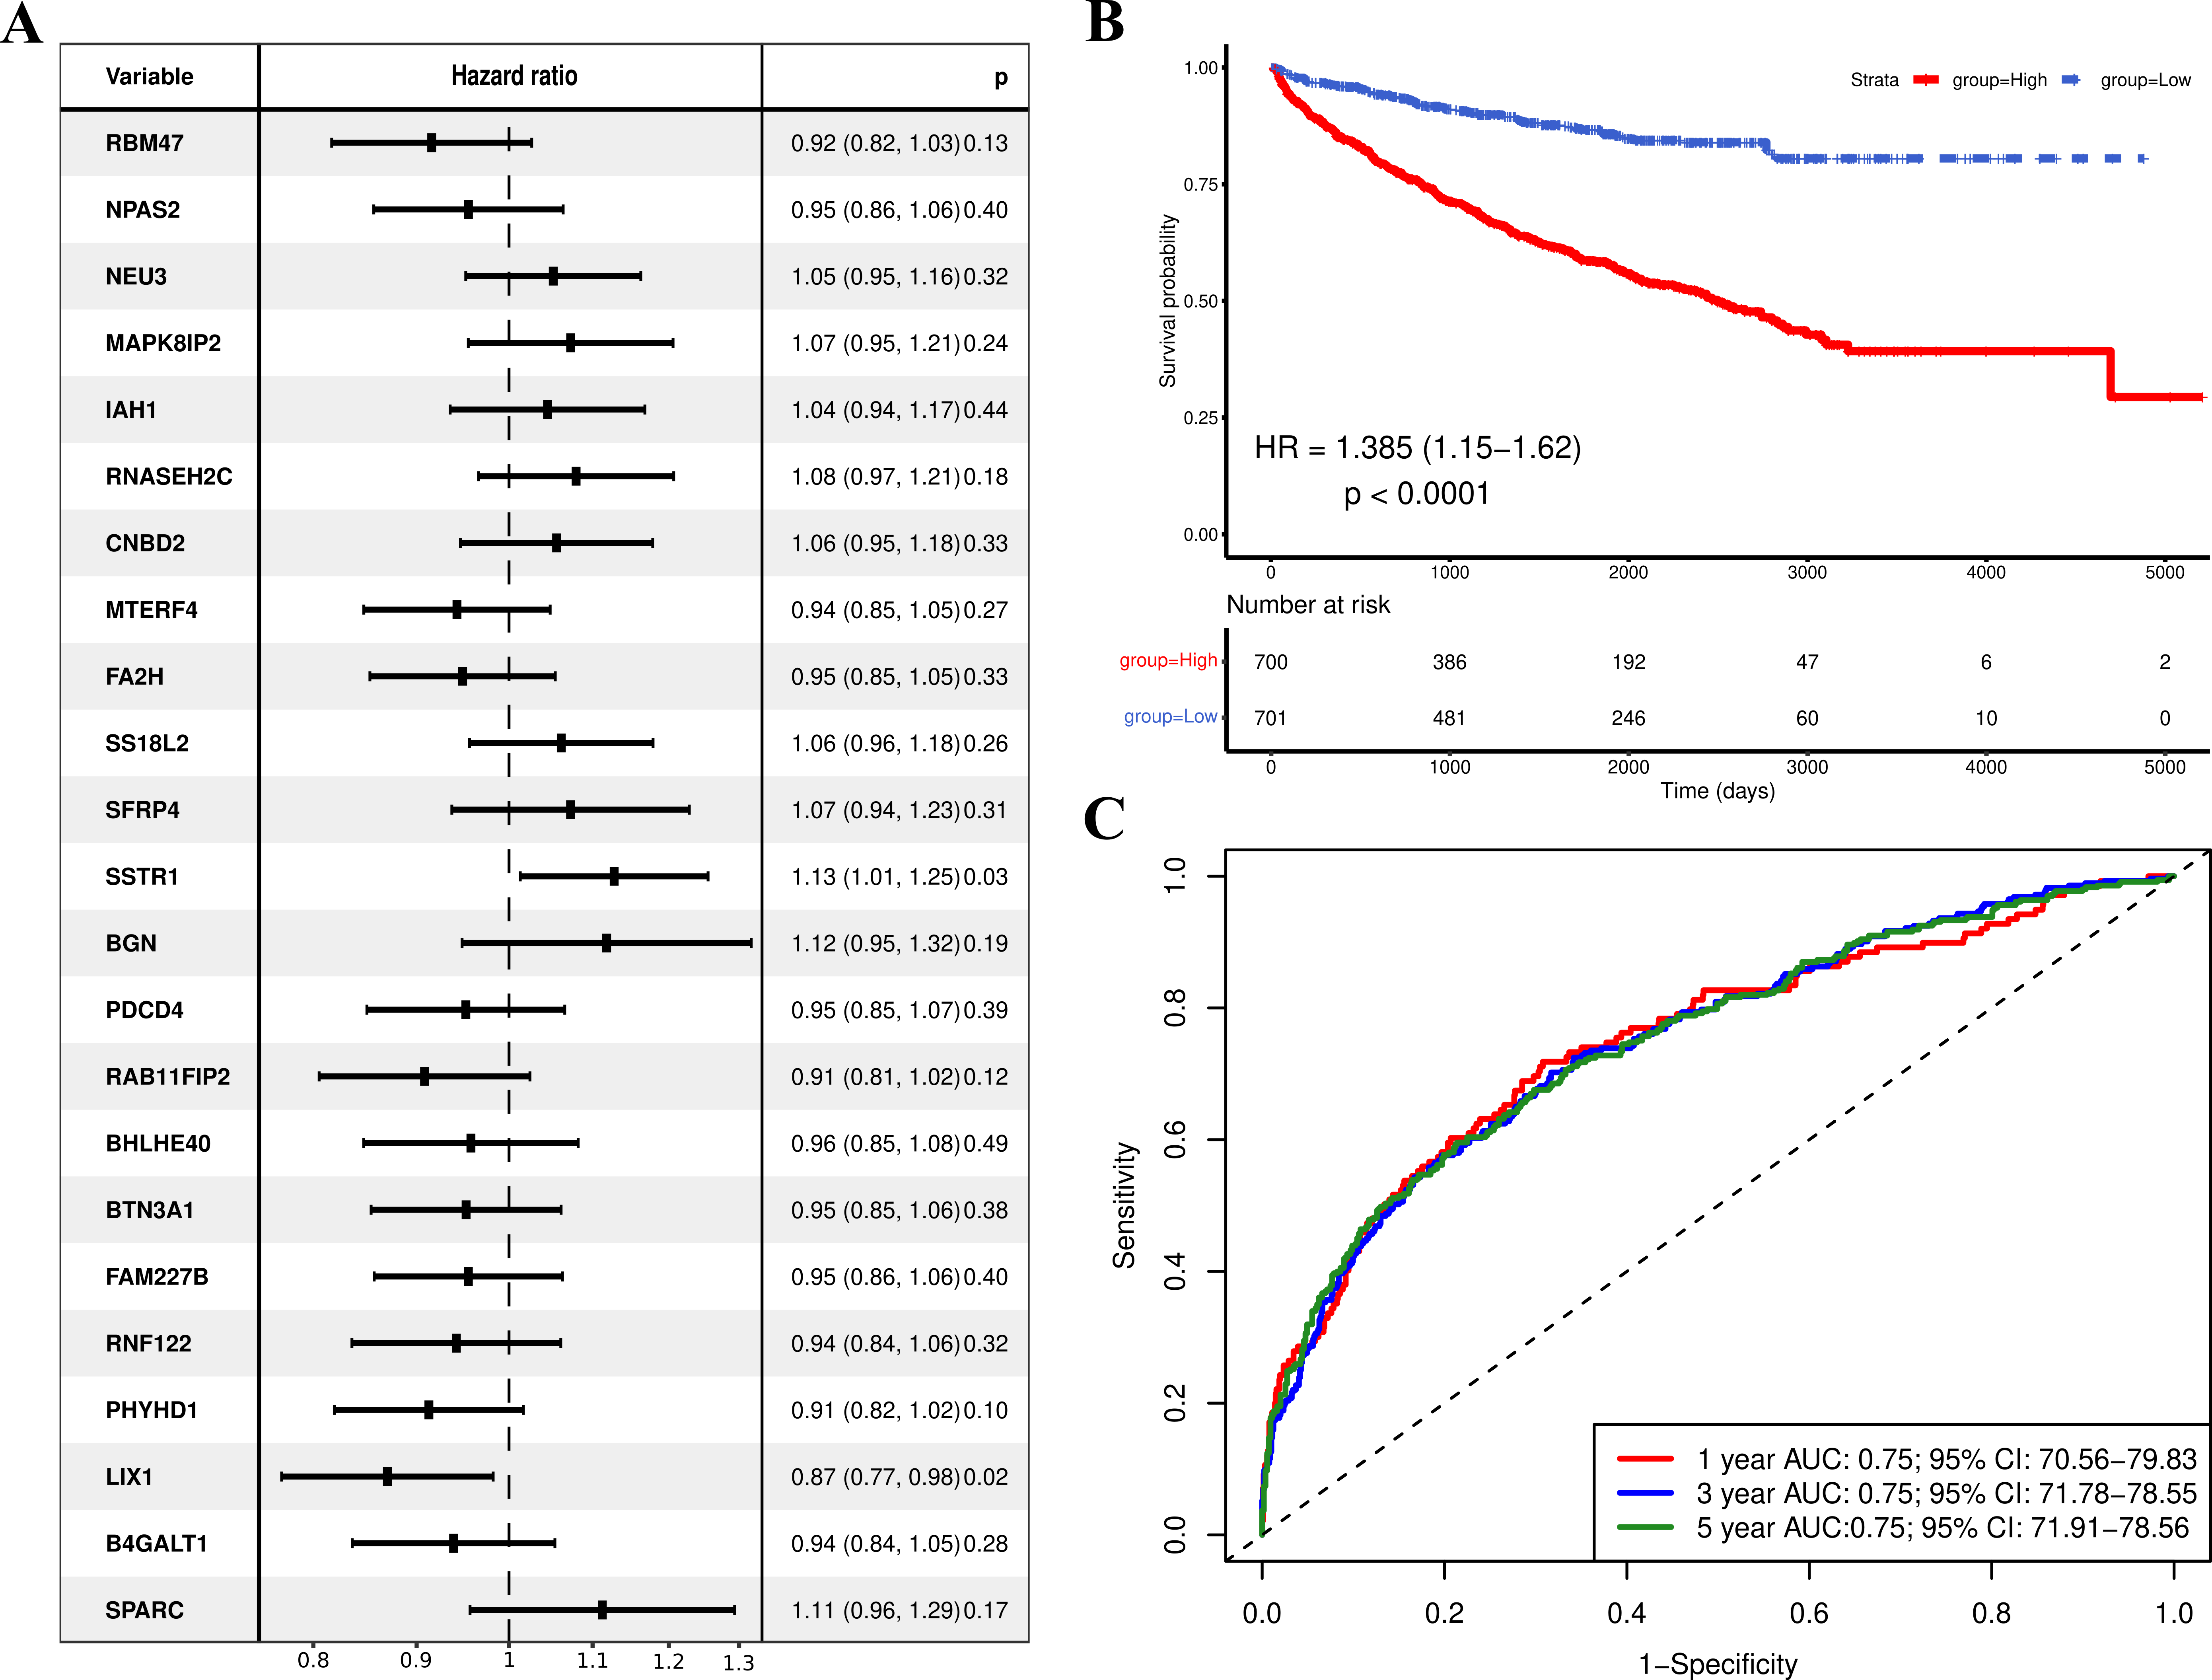
\includegraphics[width=1\textwidth]{Chapter3/Figures/Figure_1.png}
\caption[Prognostic modelling plots]{\textbf{Prognostic modelling plots} (a) Forest plot of non-zero coefficients passing Schoenfeld residual testing returned by Coxboost in the derivation dataset.  (b) Kaplan-Meier plot in the derivation dataset stratified by high-risk (red) and low-risk (blue) groups as defined by the median prognostic index cutoff point. Log-rank \textit{P} value and effect size derived from comparing high-risk to low-risk groups. (c) ROC analysis and AUC prediction accuracy of the prognostic index in the derivation dataset}\label{Figure1}
\end{figure*}

\begin{figure*}[!t]%
\centering
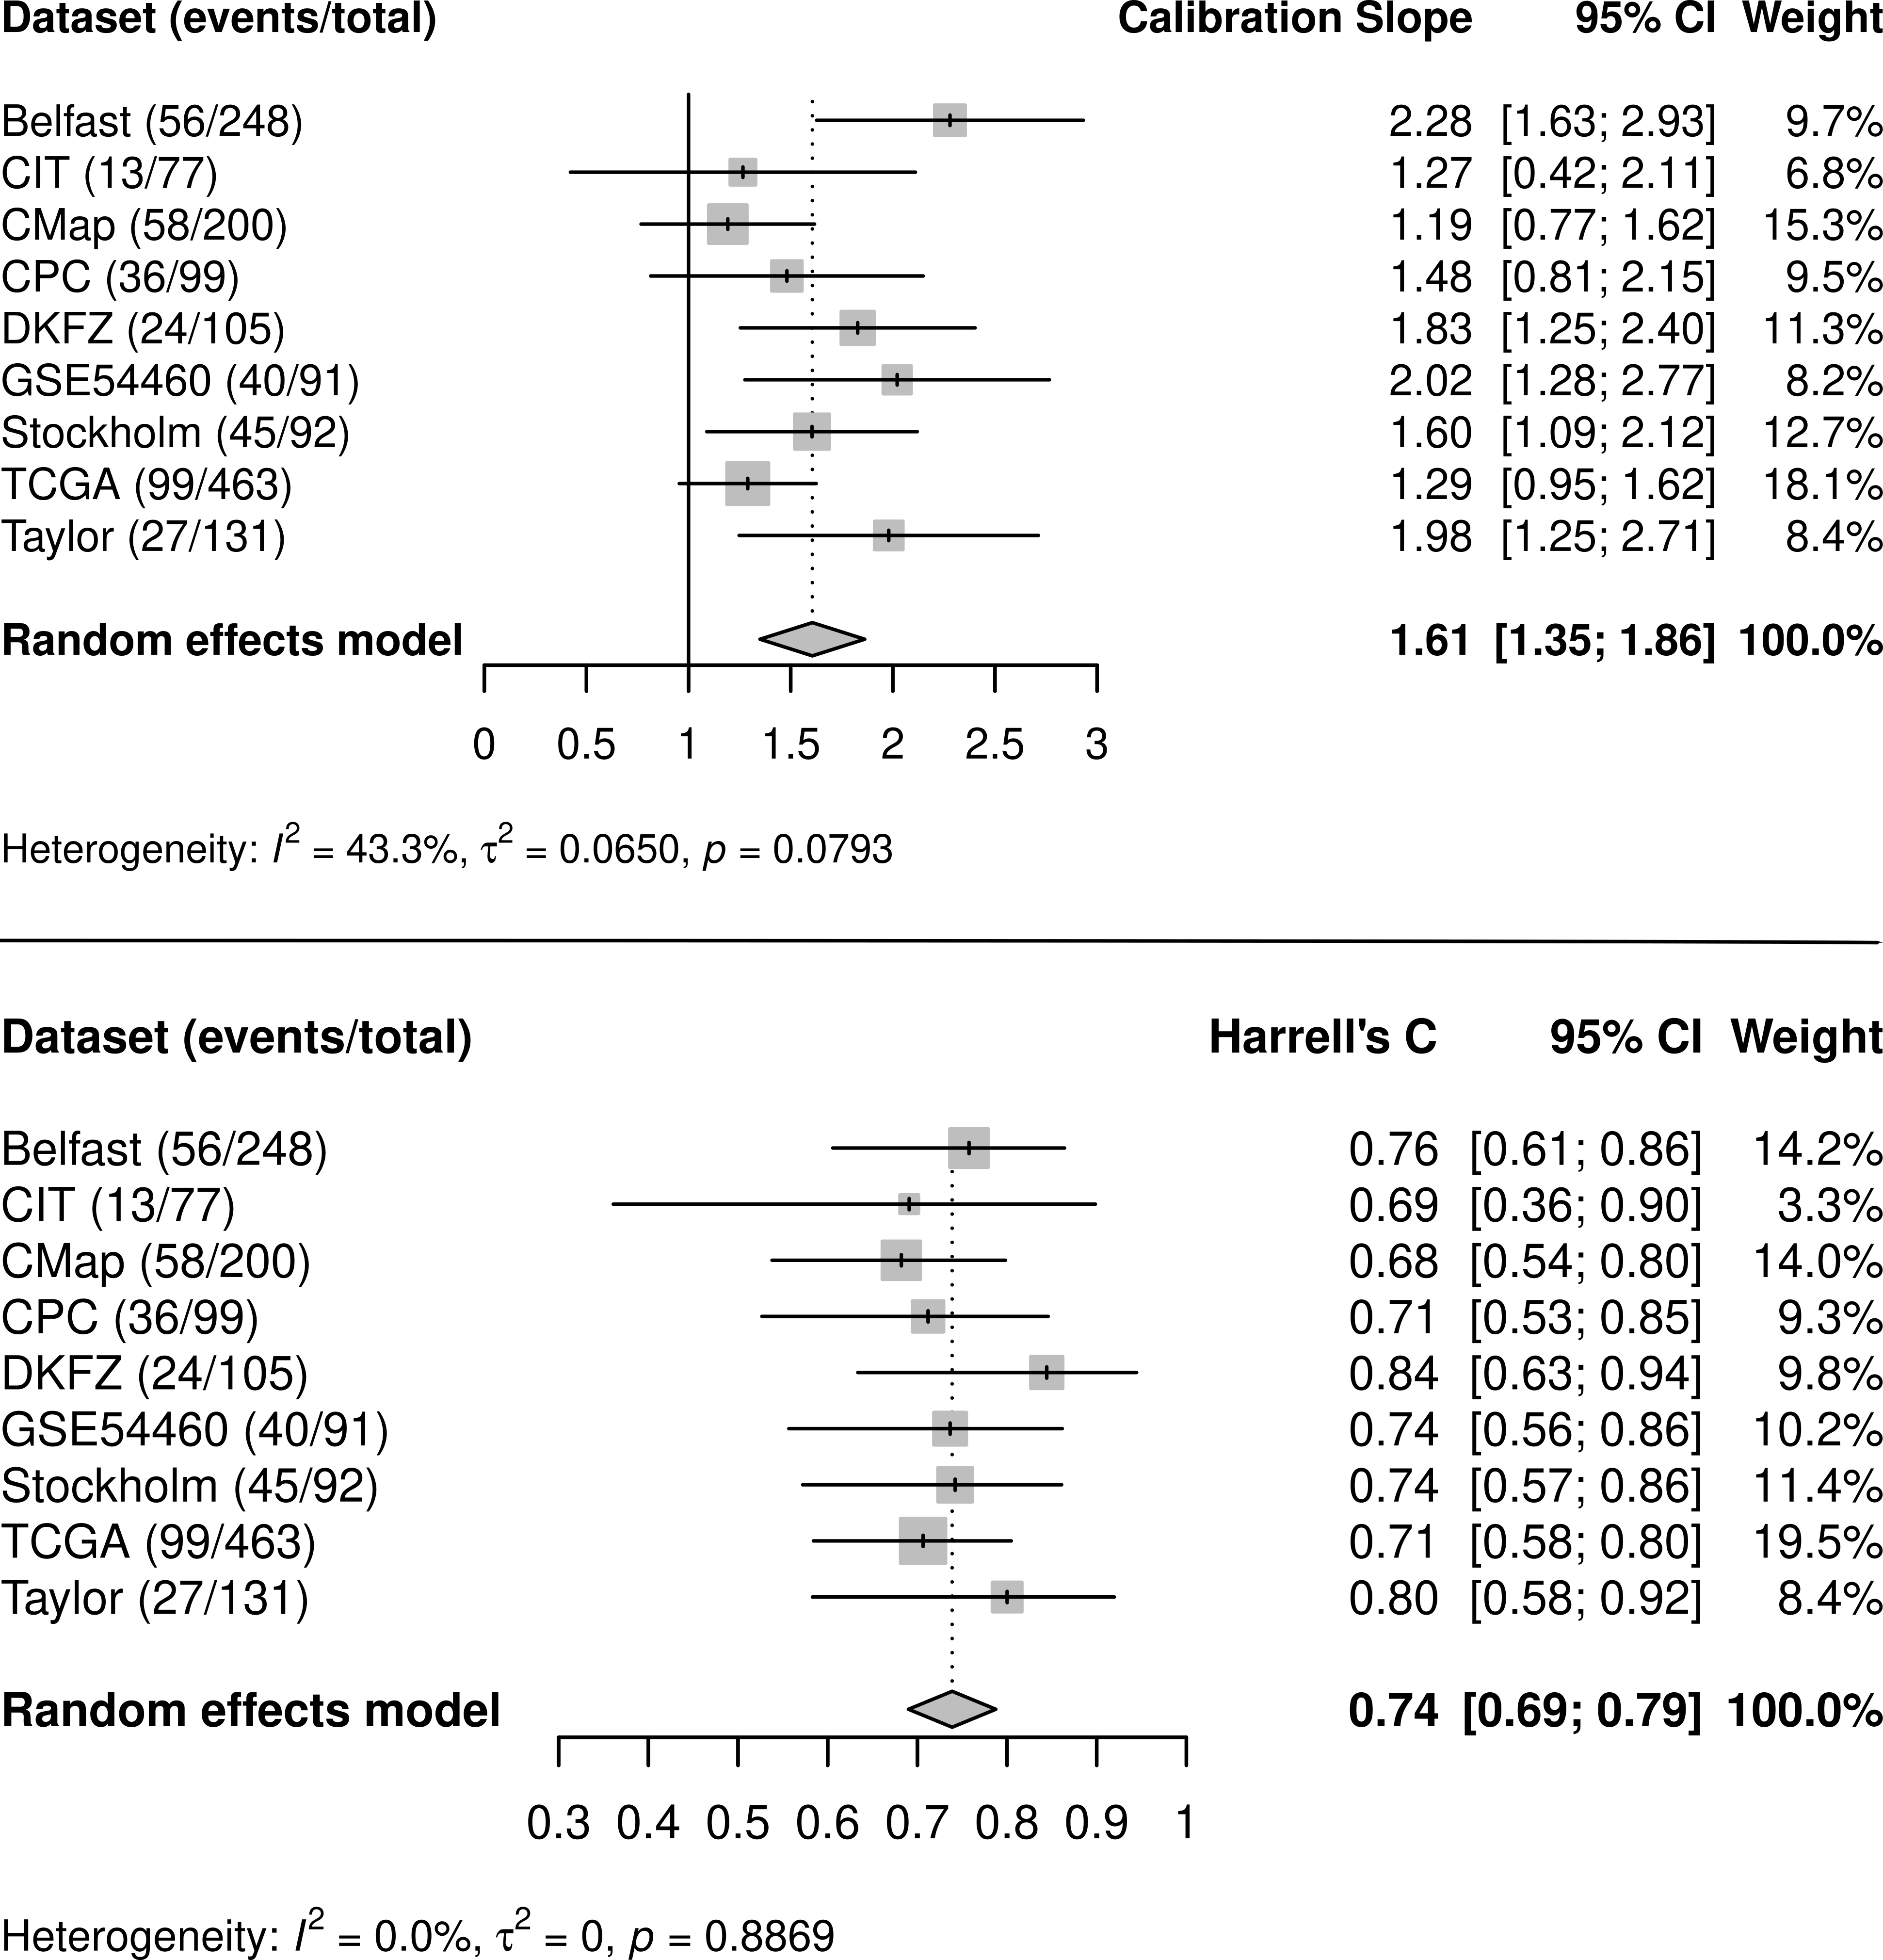
\includegraphics[width=1\textwidth]{Chapter3/Figures/Figure_2.png}
  \caption[Calibration slope, Harrell's C index forest plots]{Results from internal-external cross-validation of Cox proportional hazards model for the calibration slope (top) and Harrell's C index (bottom). Plots display each dataset's performance metric estimates and 95\% confidence intervals (squares with lines), and an overall pooled estimate obtained using random effects meta-analysis and 95\% confidence interval (diamond width encapsulates CI intervals). CI=confidence interval}\label{Figure2}
\end{figure*}

\paragraph{External Validation}
Model performance in the validation dataset remained robust, supporting the portability of the ceRNA network-derived prognostic model. The calibration slope was 1.33 (95\% CI = 0.59–2.06), which, although lower than in the derivation dataset, exceeds 1, indicating a tendency toward underfitting rather than overfitting and adequate predictive reliability (Table \ref{table2}). Discrimination was also well maintained, with time-dependent AUCs of 0.67, 0.78, and 0.87 at 1, 3, and 5 years, respectively (Figure \ref{Figure3}B), and a Harrell’s C-index of 0.71 (Table \ref{table2}). The hazard ratio in the validation cohort was 1.48, consistent with that observed during model development (Figure \ref{Figure3}A, Table \ref{table2}). Although calibration slope and hazard ratio estimates achieved statistical significance, the associated confidence intervals were wide, likely a consequence of the limited sample size in the GSE46602 validation cohort (22 BCR events among 36 patients).


%% use this setup for wide tables throughout thesis, caption + tablenotes nicely aligned. 
\begin{table*}[ht!]
\caption[Evaluation of the prognostic model in the derivation dataset and external validation dataset]{\textbf{Evaluation of the prognostic model in the derivation dataset and external validation dataset}.\label{table2}}
\begin{adjustwidth}{-0.7in}{-0in}
\tabcolsep=0pt%%
\footnotesize
\resizebox{1.2\textwidth}{!}{
\begin{tabular*}{\linewidth}{@{\extracolsep{\fill}}llllllllll@{\extracolsep{\fill}}}
  & \multicolumn{3}{c}{\textbf{Calibration slope}} & \multicolumn{2}{c}{\textbf{Chi-squared}} & & \multicolumn{3}{c}{\textbf{High risk stratum}} \\
  \cline{2-4}\cline{5-6}\cline{8-10} 
  & \textbf{coef} & \textbf{(95\% CI)} & \textbf{\textit{P} value} & \textbf{\(\chi^2_5\)} & \textbf{\textit{P} value} & \textbf{C-index}$^{1}$ & \textbf{Hazard ratio} & \textbf{(95\% CI)} & \textbf{\textit{P} value}
  \\
  \toprule
  Derivation & 1.59 & (1.41, 1.77) & 2.02e-68 & 0 & 1 & 0.73 & 1.38 & (1.15, 1.62) & 4.29e-31
  \\
  Validation & 1.33 & (0.59, 2.06) & 0.00038 & 0 & 1 & 0.71 & 1.48 & (0.52, 2.44) & 0.00257 
  \\
  \toprule
\end{tabular*}}
\end{adjustwidth}
\begin{tablenotes}
\item[$^{1}$] Harrell's C-index
\end{tablenotes}
\end{table*}


\begin{figure}[!h]%
\centering
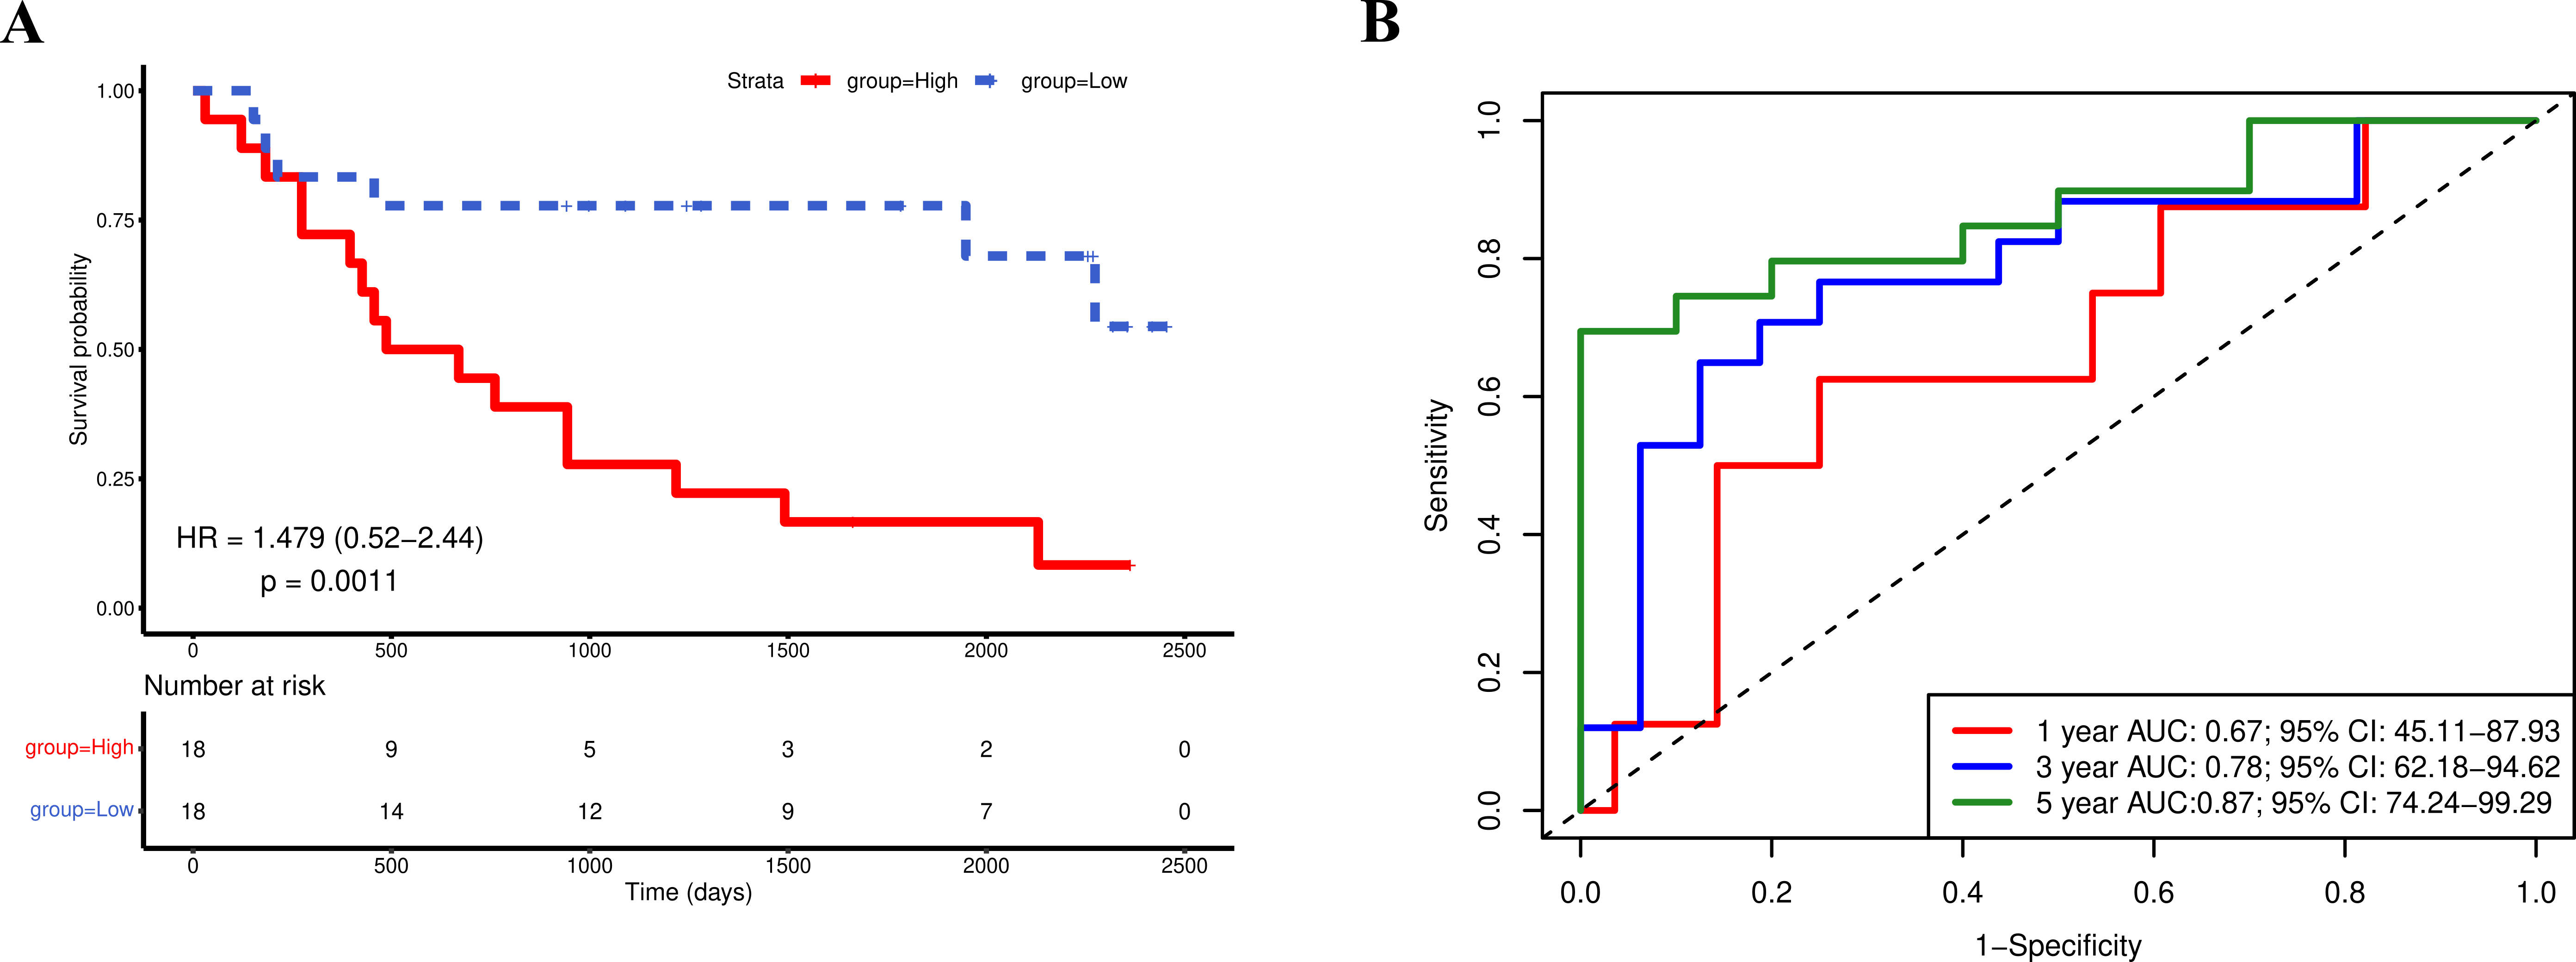
\includegraphics[width=1\textwidth]{Chapter3/Figures/Figure_3.png}
  \caption[Validation dataset plots]{(a) Kaplan-Meier plot in the validation dataset stratified by high-risk and low-risk groups as defined by the median prognostic index cutoff point, including log-rank P value. (b) ROC analysis and AUC prediction accuracy of the prognostic index in the validation dataset}
    \label{Figure3}
\end{figure}


\paragraph{Comparison to published signatures}
When comparing our model to published PCa gene signatures, we observed a lower Harrell’s C-index (0.71) in the external validation cohort compared to the highest-performing model by Long et al. (0.98) (Table \ref{table3}) \cite{Long2014}. The time-dependent AUCs of our model improved over longer follow-up periods, increasing from 0.67 at year 1, to 0.78 at year 2, and 0.87 at year 5. Notably, only two genes from our model - SFRP4 and BGN - were shared with existing published signatures, suggesting that our model captures a largely distinct set of genes associated with BCR. 
\par
The table of summary statistics generated when comparing our model to published signatures is available in Supplementary Table \ref{chp4supptable8}. 12 published signatures containing more than 28 predictors were removed from the summary statistics; \textit{NA} values for Harrell's C-index, substantial hazard ratios, large confidence intervals, and non-significant \textit{P} values were indicative of overfitting to the validation dataset, rendering comparisons infeasible.


\begin{table}[!t]
\begin{center}
\caption[Comparison to published signatures]{Signature size, Harrell's C-index and time-dependent AUC values for ceRNA network signature and published signatures in the validation dataset.\label{table3}}%
\footnotesize
\resizebox{\textwidth}{!}{
\begin{tabular*}{0.9\columnwidth}{@{\extracolsep\fill}lccccc@{\extracolsep\fill}}
  & & \textbf{Harrell's} & \multicolumn{3}{c}{\textbf{AUC (years)}} \\
  \cline{4-6}
    \textbf{Dataset} & \textbf{Genes} & \textbf{C-index} & \textbf{1} & \textbf{3} & \textbf{5} \\
    \midrule
    Agell \cite{Agell2012Nov} & 12 & 0.83 & 0.98  & 0.84  & 0.82  \\
    Bibikova \cite{Bibikova2007Jun} & 16 & 0.83 & 0.86  & 0.89  & 0.91  \\
    Bismar \cite{Cuzick2011Mar} & 12 & 0.76 &  0.83  & 0.78  & 0.81  \\
    \textbf{Digby et al.} & 23 & 0.71 & 0.67 & 0.78  & 0.87  \\
    Ding \cite{Ding2011Feb} & 4 & 0.64 & 0.55  & 0.69  & 0.80  \\
    Erho \cite{Erho2013Jun} & 19 & 0.89 & 0.99  & 0.91  & 0.95  \\
    Glinsky \cite{Glinsky2005Jun} & 11 & 0.82 & 0.81  & 0.84  & 0.81  \\
    Irshad \cite{Irshad2013Sep} & 19 & 0.89 & 0.92  & 0.96  & 0.96  \\
    Jia \cite{Jia2012} & 15 & 0.79 & 0.84  & 0.83  & 0.89  \\
    Klein \cite{Klein2014Sep} & 12 & 0.85 & 0.90  & 0.87  & 0.89  \\
    Long \cite{Long2014} & 24 & 0.98 & 0.99  & 1.00  & 1.00  \\
    Nakagawa \cite{Nakagawa2008} & 17 & 0.91 & 0.97  & 0.94  & 0.99  \\
    Olmos \cite{Olmos2012Nov} & 9 & 0.75 & 0.89  & 0.76  & 0.79  \\
    Ramaswamy \cite{Ramaswamy2003Jan} & 17 & 0.86 & 0.88  & 0.90  & 0.91  \\
    Ross \cite{Ross2011} & 6 & 0.75 & 0.86  & 0.77  & 0.81  \\
    Sharma \cite{Sharma2013Jan} & 16 & 0.78 & 0.77  & 0.83  & 0.86  \\
    Talantov \cite{Talantov2010Oct} & 3 & 0.61 & 0.52 & 0.64 & 0.61 \\
    Yu \cite{Yu2007Nov} & 14 & 0.81 & 0.86  & 0.81  & 0.88  \\
    \bottomrule
\end{tabular*}}
\end{center}
\end{table}


\subsection{Discussion}\label{sec12}
This study developed and evaluated a prognostic model to estimate the 5-year risk of BCR in PCa by identifying a common ceRNA network in PCa and enzalutamide-resistance, attempting to capture the inflection point at which BCR occurs both post-operatively and post-administration of second-generation anti-androgen drugs. ceRNA network modelling and subsequent feature selection yielded a 23-gene signature which, although sensitive to heterogeneity, obtained moderate predictive power in the external validation dataset when compared to previously published signatures. Furthermore, the 23-gene signature comprises a largely unique set of genes compared with previously published signatures, suggesting it captures distinct underlying gene expression patterns which may help elucidate the mechanistic progression of BCR.

\par

Several limitations of our work must be considered. Rich clinical metadata, including pathological T and N stages, clinical T and M stages, and age, were available only in the TCGA-PRAD cohort. In the datasets used for model development, PSA and Gleason score were the only clinical variables consistently recorded, limiting feature selection to these two predictors. Ideally, future studies should obtain complete clinical metadata for modelling, as these clinical variables are likely to influence the final set of predictors identified through feature selection.  

\par

Secondly, we were unable to generate models containing suitable predictor set sizes using alternative feature selection methods such as glmnet (LASSO, Elastic Net) and Random Forests for Survival, Regression, and Classification (RFSRC). Whilst a comparative analysis of feature selection methods would have been of interest, we ultimately selected CoxBoost, as its \textit{minstep} and \textit{maxstep} parameters allowed us to constrain the final set of predictors to an appropriate size. 

\par

Finally, our analyses revealed notable between-study heterogeneity, both at the overall model performance level and at the individual gene effect level. Internal-external cross-validation showed variability in calibration slopes and moderate heterogeneity ($I^2 = 43.3\%$) despite relatively stable discrimination performance. Complementary mixed-effects Cox modelling indicated that while most genes had stable effects across studies, a subset exhibited moderate to high variability in their prognostic associations, reflecting potential cohort-specific factors.

\par 

Attempts to directly model these study-level differences through full mixed-effects models including random slopes (e.g. $coxme(Surv(time, event) \sim gene_1 ... gene_n + (1|study))$ ) were not computationally feasible, as we encountered model convergence issues. This limitation highlights the challenge of adequately accounting for complex heterogeneity structures in high-dimensional genomic data.


\par
Regarding the genes included in our prognostic model, several support current literature, whilst others are less studied, providing novel candidates for future works. B4GALT1 is one of seven beta-1, 4-galactosyltransferase (B4GALT) genes, upregulated in bladder, lung and renal cell carcinomas \cite{Xie2016May, Xie2018May, DeVitis2019Nov}. In CRPC, B4GALT1 was found to be silenced by the androgenic enzyme AKR1C3, facilitating CRPC progression \cite{Wang2020Sep}. Our results show that B4GALT1 was downregulated in PCa and enzalutamide-resistance (-0.45 LogFC), suggesting this genes protective effect against BCR is mitigated (HR=0.94 95\% CI= 0.84-1.05). Biglycan (BGN) is secreted from extracellular matrix fibroblasts and facilitates the assembly of collagen fibrils and bone matrix \cite{Xing2015Mar}. Given that the prostate secretes numerous glycoproteins and proteoglycans \cite{Munkley2016Jun}, interest in BGN as a prognostic marker in PCa has been raised. A study demonstrated a significant association between BGN overexpression and BCR, yet when combined with clinical covariates in a multivariate model, BGN did not provide independent prognostic value \cite{Jacobsen2017Aug}. For this reason, BGN may only provide utility when combined with other markers, as utilised by the Onco\textit{type} DX prostate cancer assay \cite{Knezevic2013Oct}. Our results show overexpression (1.37 logFC) and an association with BCR (HR=1.12, 95\% CI 0.95-1.32), in agreement with Jacobsen et al. \cite{Jacobsen2017Aug}.

\par

Research by Linder et al. shows that circadian transcription factors are regulated temporally at a transcriptional level, and are dysregulated when exposed to enzalutamide in CRPC \cite{Linder2022Jun}. BHLHE40 is a circadian rhythm factor and circadian repressor; downregulation in PCa is associated with poor outcome \cite{HeidariHorestani2024Dec}. Our findings show similar downregulation (-1.95 logFC), and effect (HR=0.96, 95\% CI=0.85-1.08) in our dataset. Fatty acid 2-hydroxylase gene (FA2H) silencing accelerated gastric, colorectal and breast cancer \cite{Yao2019Mar, LiangSun2021Jan, Dai2019Oct}, increasing resistance to cisplatin and PM02734 in gastric cancer cells and human cancer cell lines, respectively \cite{Yao2019Mar, Herrero2008Dec}. Our results found FA2H to be upregulated (0.62 logFC) and protective against BCR (HR=0.95, 95\% CI=0.85-1.05), in agreement with the CMU5 prognostic signature trained and tested on the TCGA-PRAD dataset \cite{Wang2020May}. Mitogen-activated protein kinase 8 interacting protein 2 (MAPK8IP2) was found to be upregulated in multiple cancers, associated with BCR in PCa and upregulated in CRPC samples \cite{Zeng2022Nov, Cheng2020Jun}, consistent with our findings (2.35 logFC, HR=1.07 95\% CI=0.95-1.21). Neuronal PAS domain-containing protein 2 (NPAS2) is involved in anaerobic glycolysis in PCa cells; our findings support statements regarding its upregulation in PCa (0.79 logFC) \cite{Ma2023Dec}. 

\par

Upregulation of plasma membrane-associated sialidase (NEU3) has been shown to induce expression of EGR-1, AR and PSA in LNCaP cells with and without androgen, progressing PCa \cite{Kawamura2012Jan}. We found NEU3 upregulated (0.51 logFC) and associated with BCR (HR=1.05, 95\% CI=0.95-1.16). Programmed cell death protein 4 (PDCD4) is a tumour suppressor, downregulated in cancers; consistent with our findings (-0.79 logFC), capable of regulating prostate cancer cell proliferation, apoptosis, and castration resistance \cite{Zennami2019Feb}.  Phytanoyl-CoA dioxygenase domain containing 1 (PHYHD1) is downregulated in both recurrent vs. non-recurrent MCRPC and tumour vs. normal samples \cite{Li2018Feb, Su2021Sep}, similar to our findings (-0.53 logFC) in PCa and Enzalutamide-resistant samples. In a study by Khristi et al. investigating transcriptional perturbations induced by Esr2 knockdown and subsequent development of prostatic hyperplasia in \textit{R. norvegicus} \cite{Khristi2019Mar}, Family with sequence similarity 227 member B (FAM277B) was downregulated. Whilst FAM227B exhibited a protective effect against BCR (HR=0.95, 95\% 0.86, 1.06) in our datasets, its protective effect was mitigated through downregulation (-0.62 logFC). 

\par

Secreted frizzled-related protein 4 (SFRP4), a modulator of the cancer-associated Wnt pathway, is correlated with PCa aggressiveness and is an independent predictor of PCa aggressiveness in seven independent datasets \cite{Mortensen2015Nov, Horvath2004Jan, Azad2015May, Sandsmark2017Oct}. SFRP4 is included in multiple prognostic signatures \cite{Feng2022Jan, Yimamu2022Dec}, including the commercially available Onco\textit{type} DX test \cite{Knezevic2013Oct}. We found SFRP4 to be upregulated (1.40 logFC) and associated with BCR (HR=1.07, 95\% CI=0.94-1.23). Secreted protein, acidic, rich in cysteine (SPARC) expression is highly expressed in patients experiencing metastases after radical therapy and associated with higher Gleason scores \cite{HutchSPARC, Lopez-Moncada2019Nov}. Our results contradict these studies (-0.48 logFC), yet corroborate findings from several studies demonstrating SPARC expression is downregulated in PCa \cite{Chekhun2024Feb, Shin2013Aug}. Our results demonstrate Limb Expression 1 (LIX1) is downregulated (-2.48 logFC), mitigating its protective effects against BCR (HR=0.87, 95\% CI=0.77-0.98), consistent with recent work by Fan et al. \cite{Fan2025Feb}. 

\par

Whilst some genes in our prognostic signature remain understudied in PCa, their broader functions and associations with cancers warrant discussion. BTN3A1, a butyrophilin family membrane protein involved in T-cell activation and immune regulation, has been implicated as a tumour suppressor in breast and non–small cell lung cancer, where lower expression is associated with worse outcomes \cite{Liang2021Aug}. We report similar trends (-1.41 logFC, HR=0.95, 95\% CI=0.85-1.06) in PCa. RBM47, an RNA-binding protein, functions as a tumour suppressor by regulating splicing and stabilising antitumor transcripts in breast cancer \cite{Vanharanta2014Jun}. Similarly, in renal cell carcinoma, RBM47 acts as a tumour suppressor by inhibiting proliferation, migration, and invasion, with higher expression correlating with improved prognosis \cite{Wang2023Dec}. Our results show upregulation of RBM47 (0.36 logFC) with a protective effect against BCR (HR=0.92, 95\% CI=0.82-1.03). Rab11 family-interacting protein 2 (RAB11FIP2) overexpression is associated with tumour angiogenesis and poorer prognosis in colorectal cancer \cite{Dong2018Dec, Xu2016Feb}. Our results demonstrate downregulation in PCa with higher expression associated with a protective effect against BCR (-0.76 logFC, HR=0.91, 95\% CI=0.81-1.02). The mitochondrial transcription termination factor 4 (MTERF4) knockdown induces apoptosis, whilst overexpression promotes cell proliferation in HeLa cells \cite{Yu2011May}. We observed upregulation and a protective effect against BCR in our data (1.04 logFC, HR=0.94, 95\% CI=0.85-1.05).

\par 

Cyclic nucleotide binding domain containing 2 (CNBD2) is a prognostic marker in pancreatic cancer, where lower expression is associated with poor outcomes \cite{Uhlen2017Aug}. Our results demonstrate low levels of upregulation are associated with BCR (0.45 logFC, HR=1.06, 95\% CI=0.95-1.18). Overexpression of the ring finger protein 122 (RNF122) gene in glioblastoma samples and cell lines is associated with tumour progression via the  JAK2/STAT3/c‐Myc signaling pathway \cite{Xiao2024Sep}. We observed downregulation (-0.59 logFC), mitigating the protective effect of the gene (HR=0.94, 95\% CI 0.84, 1.06). SS18-like 2 protein (SS18L2) knockdown in triple-negative breast cancer cell lines induces G2/M arrest and apoptosis \cite{Yedier-Bayram2022Aug}. No current literature links SS18L2 to prostate cancer, thus our findings showing upregulation of SS18L2 in prostate cancer and enzalutamide-resistant cell lines (0.54 logFC) and higher expression associated with BCR (HR=1.06, CI 95\% 0.96, 1.18) warrant further investigation.
\par


For the remaining genes IAH1 and RNASEH2B, little is currently known about their role in cancers. Their inclusion in the prognostic signature underscores the hypothesis-generating value of our model; they represent promising candidates for functional follow-up studies, which could uncover novel roles in tumour progression, treatment response, or disease etiology.

\subsection{Conclusion}\label{sec13}
In summary, we integrated the transcriptomic profiles of prostate cancer patients and enzalutamide-resistant LNCaP cell lines at the circRNA, miRNA, and mRNA levels to construct a competing endogenous RNA network as a prognostic tool for biochemical recurrence. By leveraging regulatory information from the network, rather than relying on traditional machine learning dimension reduction techniques, we derived a biologically informed gene signature associated with recurrence. We further provide robust model evaluation techniques, offering a reproducible framework for future studies in prostate cancer prognosis.


\subsection*{Acknowledgements}

The authors thank Dr. Marvin Lim and Dr. Elaine Kenny for generating sequencing data on LNCaP cell lines.

\subsection*{Author contributions statement}

\textbf{B.D}: Conceptualization, Methodology, Software, Formal Analysis, Data Curation, Writing - Original Draft. \textbf{S.P.F}: Resources, Writing - Review \& Editing, Supervision. \textbf{P.\'{O}.B}: Conceptualization, Writing - Review \& Editing, Supervision, Funding Acquisition.


\subsection*{Competing interests}
The authors declare no competing interests.

\subsection*{Data Availability}
The following publicly available resources were used to obtain circRNA, miRNA and mRNA expression datasets: \href{https://portal.gdc.cancer.gov}{GDC Data Portal}, \href{https://www.ncbi.nlm.nih.gov/geo}{Gene Expression Omnibus}, \href{https://www.ebi.ac.uk/biostudies/arrayexpress}{ArrayExpress}, \href{http://bioinfo.jialab-ucr.org/PCaDB/}{PCaDB}. LNCaP sequencing data generated for this study are available at GSE312115 using the access token erupkycyvpkvvoj and Supplementary File \hyperlink{chp4suppfile1}{1}, respectively. All code used in the manuscript analysis is freely available on \href{https://github.com/BarryDigby/pca_network}{Github}.

\subsection*{Funding}
This research was funded by Science Foundation Ireland, grant number 18/CRT/6214.


\subsection{Supplementary Tables}

% Figures
\renewcommand{\thefigure}{\chapternum.S\arabic{figure}}
\setcounter{figure}{0}

% Tables
\renewcommand{\thetable}{\chapternum.S\arabic{table}}
\setcounter{table}{0}


\begin{table*}[ht!]
\caption[Prostate cancer datasets used for network construction]{Prostate cancer datasets used for differential expression testing and subsequent network construction.}
\label{chp4supptable1}
\footnotesize
\resizebox{\textwidth}{!}{
	\begin{tabular}{lcccr}
	\toprule 
	\textbf{Data type} & \shortstack{\textbf{Sample size}\\\textbf{(tumor/normal)}} & \textbf{Series} & \textbf{Platform} & \textbf{Reference} 
	\\
	\toprule 
	circRNA & 10/0 & \href{https://www.ncbi.nlm.nih.gov/geo/query/acc.cgi?acc=GSE113153}{GSE113153} & GPL21825 & \cite{Yang2019}
	\\
	miRNA & 100/28 & \href{https://www.ncbi.nlm.nih.gov/geo/query/acc.cgi?acc=GSE21036}{GSE21036} & GPL8227 & \cite{Taylor2010Jul}
	\\ 
	miRNA & 20/20 & \href{https://www.ncbi.nlm.nih.gov/geo/query/acc.cgi?acc=GSE23022}{GSE23022} & GPL8786 & \cite{Wach2012}
	\\
	miRNA & 21/21 & \href{https://www.ncbi.nlm.nih.gov/geo/query/acc.cgi?acc=GSE36803}{GSE36803} & GPL8786 & \cite{Lin2013} 
	\\ 
	miRNA & 50/10 & \href{https://www.ncbi.nlm.nih.gov/geo/query/acc.cgi?acc=GSE45604}{GSE45604} & GPL14613 & \cite{CasanovaSalas2014} 
    \\
	miRNA & 53/4 & \href{https://www.ncbi.nlm.nih.gov/geo/query/acc.cgi?acc=GSE46738}{GSE46738} & GPL8786 & \cite{Leite2015}  
	\\ 
	miRNA & 498/52 & \href{https://portal.gdc.cancer.gov/repository}{TCGA} & Illumina HiSeq & \cite{Grossman2016}
	\\
	mRNA & 498/52 &  \href{https://portal.gdc.cancer.gov/repository}{TCGA} & Illumina HiSeq & \cite{Grossman2016} 
	\\
	\toprule
	\end{tabular}}
\end{table*}



\begin{table*}[hbt!]
\caption[Enzalutamide datasets used for network construction]{Enzalutamide datasets used for differential expression testing and subsequent network construction. Clone 1 (high ENZ-resistance), Clone 9 (moderate ENZ-resistance).}
\label{chp4supptable2}
\footnotesize
\resizebox{\textwidth}{!}{
	\begin{tabular}{llllr}
	\toprule
	\textbf{Data type} & \shortstack{\textbf{Description of LNCaP samples}\\\textbf{(\textit{n} per subgroup)}} & \textbf{Series} & \textbf{Platform} & \textbf{Reference} 
	\\
	\toprule
	circRNA & Clone 1, Clone 9, Control (n=3) & \href{https://www.ncbi.nlm.nih.gov/geo/query/acc.cgi?acc=GSE118959}{GSE118959} & GPL21825 & \cite{Greene2019,Lim2021Dec}
	\\
	miRNA & Clone 1, Clone 9, Control (n=3) & \href{https://www.ncbi.nlm.nih.gov/geo/query/acc.cgi?acc=GSE312115}{GSE312115} & Illumina MiSeq & \textit{Digby et al.}
	\\
	mRNA & 21, 14, 7, 0 days ENZ treated (n=3) & \href{https://www.ncbi.nlm.nih.gov/geo/query/acc.cgi?acc=GSE143408}{GSE143408} & GPL25684 & \cite{Tousignant2020}
	\\
	mRNA & 6 months ENZ treated, control (n=4) & \href{https://www.ncbi.nlm.nih.gov/geo/query/acc.cgi?acc=GSE78201}{GSE78201} & GPL10558 & \cite{Kregel2016}
	\\
	mRNA & ENZ treated, ENZ sensitive (n=4) & \href{https://www.ncbi.nlm.nih.gov/geo/query/acc.cgi?acc=GSE88752}{GSE88752} & GPL11154 & \cite{Li2018}
	\\
	mRNA & Clone 1, Clone 9, Control (n=3) & \textit{in-house} & Illumina NovaSeq & \textit{N/A}
	\\
	\toprule
	\end{tabular}}
\end{table*}




\begin{table*}[hbt!]
\caption[Summary of datasets used for prognostic signature development and validation]{Datasets used for prognostic model development and external validation (GSE46602). Sample sizes are reported as (BCR events/total) following removal of patients with missing BCR information.}
\label{chp4supptable3}
\footnotesize
\resizebox{\textwidth}{!}{
	\begin{tabular}{llllr}
	\toprule
	\textbf{Dataset} & \textbf{BCR events/total} & \textbf{Series} & \textbf{Platform} & \textbf{Reference}
	\\
	\toprule
	Belfast & 56/248 & \href{https://www.ncbi.nlm.nih.gov/geo/query/acc.cgi?acc=GSE116918}{GSE116918} & GPL25318 &  \cite{Jain2018}
	\\
        CIT & 13/77 & \href{https://www.ncbi.nlm.nih.gov/geo/query/acc.cgi?acc=GSE54460}{GSE54460} & GPL11154 & \cite{Long2014}
        \\
        CMap & 58/200 & \href{https://www.ncbi.nlm.nih.gov/geo/query/acc.cgi?acc=GSE94767}{GSE94767} & GPL5175 & \cite{Luca2018}
        \\
        CPC & 36/99 & \href{https://www.ncbi.nlm.nih.gov/geo/query/acc.cgi?acc=GSE107299}{GSE107299} & GPL16686 & \cite{Sinha2019Mar}
        \\
        DKFZ & 24/105  & \href{https://ega-archive.org/studies/EGAS00001002923}{EGAS00001002923} & GPL11154 & \cite{Gerhauser2018}
        \\
        GSE46602 & 14/36 & \href{https://www.ncbi.nlm.nih.gov/geo/query/acc.cgi?acc=GSE46602}{GSE46602} & GPL570 & \cite{Mortensen2015Nov}
        \\
        GSE54460 & 40/91 & \href{https://www.ncbi.nlm.nih.gov/geo/query/acc.cgi?acc=GSE54460}{GSE54460} & GPL11154 & \cite{Long2014}
        \\
        Stockholm & 45/92 & \href{https://www.ncbi.nlm.nih.gov/geo/query/acc.cgi?acc=GSE70769}{GSE70769} & GPL10558 & \cite{RossAdams2015}
        \\
        TCGA & 99/463 & \href{https://portal.gdc.cancer.gov/repository}{TCGA} & Illumina HiSeq & \cite{Grossman2016}
        \\
        Taylor & 27/131 & \href{https://www.ncbi.nlm.nih.gov/geo/query/acc.cgi?acc=GSE21034}{GSE21034} & GPL5188 & \cite{Taylor2010Jul}
        \\
    \toprule
	\end{tabular}}
\end{table*}


\begin{table*}[h!]
  \centering
  \caption[Prognostic signatures used for comparison in the external validation dataset]{PCa prognostic signatures used for comparison in the external validation dataset}
  \label{chp4supptable4}
  \footnotesize
  \begin{adjustbox}{max width=\textwidth}
  \begin{tabular}{llr}
  \toprule 
  \textbf{Signature} & \textbf{Genes} & \textbf{Reference}
  \\
  \toprule 
  Agell & 12 &  \cite{Agell2012Nov}
  \\
  Bibikova & 16 & \cite{Bibikova2007Jun}
  \\ 
  Bismar & 12 & \cite{Bismar2006Jan}
  \\ 
  Cuzick & 31 & \cite{Cuzick2011Mar}
  \\
  Ding & 4 & \cite{Ding2011Feb}
  \\ 
  Erho & 19 & \cite{Erho2013Jun}
  \\ 
  Glinsky & 11 & \cite{Glinsky2005Jun}
  \\ 
  Irshad & 19 & \cite{Irshad2013Sep}
  \\
  Jia & 15 & \cite{Jia2012}
  \\
  Kamoun & 36 & \cite{Kamoun2018}
  \\ 
  Klein & 12 & \cite{Klein2014Sep}
  \\
  Li & 160 & \cite{Li2021May}
  \\
  Long & 24 & \cite{Long2014}
  \\
  Luca & 45 & \cite{Luca2018}
    \\
  Mo & 93 & \cite{Mo2018Apr}
    \\ 
  Nakagawa & 17 & \cite{Nakagawa2008} 
    \\
  Olmos & 9 & \cite{Olmos2012Nov} 
    \\
  Penney & 157 & \cite{Penney2011Jun} 
    \\
  Planche & 36 & \cite{Planche2011} 
    \\
Ramaswamy & 17 & \cite{Ramaswamy2003Jan} 
  \\
Ramos-Montoya & 222 & \cite{Ramos-Montoya2014May} 
  \\
Ross & 6 & \cite{Ross2011} 
  \\
Ross-Adams & 100 & \cite{Ross-Adams2015Jul} 
  \\
Sharma & 16 & \cite{Sharma2013Jan} 
  \\
Sinnott & 30 & \cite{Sinnott2017Jan} 
  \\
Talantov & 3 & \cite{Talantov2010Oct} 
  \\
Varambally & 44 & \cite{Varambally2005Nov}
  \\
Wu & 29 & \cite{Wu2013Apr} 
  \\
Yang & 28 & \cite{Yang2018May} 
  \\
Yu & 14 & \cite{Yu2007Nov} 
  \\
  \toprule
  \end{tabular}
  \end{adjustbox}
  \end{table*}


\clearpage

\begin{adjustwidth}{-0cm}{-0cm}
    \begin{longtblr}[
        entry = {Frequency of genes selected over 200 bootstrap samples},
        caption = {Frequency of genes selected by Coxboost over 200 bootstrap samples and passing Schoendfeld residuals filtering. Genes included in the final model are colored red.},
        label = {chp4supptable5}
        ]{
        colspec = {r X[4,l]},%% put weights for column width in []
        rowhead = 1
        }
        \hline
        \textbf{Frequency} & \textbf{Genes} \\
        \hline
        118 & gleason\_score \\
        105 & \textcolor{red}{RNASEH2C} \\
        102 & \textcolor{red}{SSTR1} \\
        94 & \textcolor{red}{SPARC} \\
        84 & \textcolor{red}{BGN} \\
        68 & \textcolor{red}{LIX1} \\
        60 & \textcolor{red}{NEU3} \\
        57 & \textcolor{red}{SFRP4} \\
        56 & \textcolor{red}{BHLHE40} \\
        54 & \textcolor{red}{SS18L2} \\
        52 & DCAF4L1 \\
        49 & \textcolor{red}{PHYHD1} \\
        48 & \textcolor{red}{PDCD4} \\
        46 & ST3GAL3 \\
        44 & TPCN2 \\
        43 & \textcolor{red}{CNBD2} \\
        42 & CELF5, SMCO3 \\
        41 & \textcolor{red}{FAM227B} \\
        39 & \textcolor{red}{RAB11FIP2} \\
        37 & POLR2L \\
        35 & LMO2, \textcolor{red}{NPAS2} \\
        34 & \textcolor{red}{BTN3A1}, DOCK6, PRDM1, ZNF287 \\
        33 & LRIF1, \textcolor{red}{RNF122} \\
        32 & HLX, \textcolor{red}{MTERF4} \\
        31 & REG4, SLC9B1, SRF \\
        30 & GLIPR2, \textcolor{red}{IAH1} \\
        29 & SLX4IP \\
        28 & COX6C, \textcolor{red}{FA2H}, NUS1 \\
        26 & RPIA \\
        25 & DLG3, MIEN1 \\
        24 & ACVRL1, \textcolor{red}{RBM47}, SLC35G1 \\
        23 & DDAH1, SLC2A4, SLC39A14, ZFPL1 \\
        22 & CDK17 \\
        21 & \textcolor{red}{MAPK8IP2}, SLCO5A1, ZNF623 \\
        20 & ZNF518B \\
        19 & HIC2, NDUFA1, TBC1D8, TMEM63C, TRAM2, TRIB1, UROS, ZNF268, ZNF804A \\
        18 & ATAD3C \\
        17 & CDCA7L, KIF21A, PRR13 \\
        16 & \textcolor{red}{B4GALT1}, BACE2, DHTKD1, RFXAP, TMEM151A \\
        15 & CDKN1A, DHX38, FOXL2, KCNC2 \\
        14 & AGRN, B3GAT1, TMC5 \\
        13 & CTHRC1, DPT, GSK3A, IGSF22, KCNS3, YKT6 \\
        12 & CHRM1, DHX40, GLP1R, MAEA, PAPSS1, PLIN1, ZBTB3 \\
        11 & FBXO43, OGFOD1, REPS1, RHOU, STARD3NL, TMSB10 \\
        10 & ALG9, C14orf39, C2orf68, CHRM3, CLPTM1, DUSP3, SARNP, TG, ZFR, ZNF138 \\
        9 & C1orf53, COX20, CRTC1, DNASE1L1, FAM117B, GCC1, GTF3C1, ITSN1, KAZN, LZIC, SH3RF1, SLC28A3, YPEL1, ZNF561 \\
        8 & ABCA12, ACAN, DECR1, DEDD, GPR37, LAMC1, MZB1, PACS1, POFUT2, TMEM54, TNS4 \\
        7 & ADGRG6, ATP1B3, BICD2, CRISPLD2, CSNK2A2, ELAVL2, EPSTI1, INHBB, KDM8, KL, LETMD1, MKRN1, MOCOS, MSR1, MUC6, NET1, RAB34, SCNN1G, SCRIB, WDR93 \\
        6 & CALML5, CBLB, ECHDC3, GBA2, HBQ1, HEY2, IGSF9B, KMO, MASP1, NSL1, RNF214, RPP30, SNAI2, STK35, TMEM164, TMEM44, TMF1, TRIM24, WASF2, ZNF664 \\
        5 & ABHD10, ANKFY1, ANXA3, CATSPERG, CDK10, COX10, FADS2, FBXO45, HS6ST1, JAG2, KREMEN1, OPA1, PABPC1L2A, PAPPA, PFKFB2, PGM2L1, PILRA, PPP4R4, SEC31B, SIAH3, SLC22A23, SLC22A3, STARD5, TEAD3, TMPRSS11F, USO1, WNT2B, ZNF830 \\
        4 & AKAP10, AQP4, C1orf216, CCDC120, CCNT2, CFAP44, EIF4G2, EPHA8, FADS1, GLUL, GRHL2, IPO11, KCNK9, LPIN1, LRTM2, MINK1, NAV3, NELFB, NFKBIL1, ORMDL1, PADI4, PPARGC1A, PPM1F, PPP3CB, SLC13A3, SLC25A21, SLC39A5, SP5, SUOX, TMEM192, TTC31 \\
        3 & ABHD13, ADAMTSL3, ANXA2, ARL8A, ARNT, ASCC3, ASPHD1, ATP6AP1, BRSK2, BTF3L4, CAMKV, CDCP1, CEP85L, CHST4, CLDN14, COL19A1, CPSF4, DSC3, ECHDC2, EFNA1, EHF, FAM43B, FMO5, FRMD5, GJB2, GMCL1, GNA14, GSAP, HBS1L, HCST, IL15RA, INSM2, IPO5, KIFC2, LRRC28, METAP1, MMP9, MNAT1, NAPA, NCALD, PHLDA3, PLAT, PWP1, RBL1, RIF1, SCAMP5, SGSM2, SIX4, SLC2A1, SNRPE, TCEANC2, THYN1, ZFP28, ZNF768 \\
        2 & ABRACL, ACSS2, ACTR3, AJAP1, ALX4, ASB4, BUD31, C3orf62, CACNA2D2, CACNB3, CENPQ, COL2A1, CTDSP2, DLGAP2, DRAM1, EBF2, EIF2B1, EYS, FMOD, GALNT10, GALNT11, HIC1, HMGCLL1, HNRNPA0, IBA57, IPO8, KIF20B, LGI3, LMTK2, LONRF1, LRRC61, LTA4H, MAK16, MCFD2, MCM3, MEIS1, MIOS, MIS12, MTERF2, NCDN, NDE1, NFIC, NFXL1, PER1, PLEKHM3, PPA2, RNMT, RPE65, RPS6KL1, SCFD1, SLC12A7, SLC5A9, SLCO3A1, SMG9, SRRD, SYNC, TH, THUMPD2, TOE1, TSC22D4, TTLL5, TTPA, TXLNB, UBE2E3, ULK1, UQCRB, USPL1, VDR, WDR59, WWTR1, YWHAG, ZDHHC18, ZMYM1, ZNF142, ZNF267, ZNF347, ZNF460, ZNF532, ZNF546 \\
        1 & ACVR2B, AKIRIN1, ANKRD53, ANXA5, ARSB, ASB1, BICC1, C19orf81, C2orf49, CAMLG, CATSPERB, CCND3, CEP120, CNIH4, CNP, COPB2, CUL5, CYP2E1, DAGLB, DDX3Y, DDX5, DENND4B, DFFA, DIRAS2, DYNC2LI1, EAF1, EDAR, EFHC1, EIF5, EMILIN2, ENOSF1, EPHA10, EPHB3, ESD, F10, FAM171A1, FBXO24, FRAT1, GIGYF1, GIT1, GPR87, GSR, HABP2, HEYL, HIF1A, HINFP, HPD, HSD11B1, IFI27L1, IFRD1, IFT81, IGDCC3, ING5, INPP5E, INPP5F, ISL1, ITGA5, KLK5, LEF1, LINGO1, LYRM7, MAG, MAOB, MARVELD2, MDH1B, ME1, MED6, MFSD10, MGAT5B, MORC2, MSANTD1, MTMR9, MUC4, NDUFA10, NKAIN1, NLRP9, NOL7, NRG4, NSRP1, NUMBL, NUP43, NXPH1, PBLD, PCDH1, PCDHB10, PCNP, PDIK1L, PHF19, PKHD1L1, PM20D2, PON2, PREB, PRMT9, PRPF39, PRRX1, QRFPR, QRSL1, RABIF, RALY, RASSF2, REN, RIT2, RNF168, RSRP1, SLC22A2, SLC25A37, SLC35F3, SLC36A4, SLC7A9, SRSF6, STKLD1, STRIP2, STX7, SYT7, TBCC, TMEM109, TMEM150C, TOR1B, TRIM59, TRPC4, TRUB1, UBA1, VPS54, ZC2HC1C, ZNF134, ZNF212, ZNF281, ZNF585B, ZNF706, ZNF791, ZNF862, ZRANB2 \\
        \hline
    \end{longtblr}
\end{adjustwidth}



\begin{table*}[t]
  \begin{adjustwidth}{-0.0in}{0in}
  \centering
  \caption[Model performance across internal-external cross-validation folds]{Prognostic model performance across internal-external cross-validation folds. Regular font study names represent the derivation dataset, whilst study names in bold represent the validation dataset. The derivation dataset represents a combination of all studies except the study listed, which is reserved as the validation dataset.}
  \label{chp4supptable6}
  \resizebox{1.05\linewidth}{!}{
  \begin{tabular}{llllllllll}
  \\
  & \multicolumn{3}{c}{\textbf{Calibration slope}} & \multicolumn{2}{c}{\textbf{Chi-squared}} & & \multicolumn{3}{c}{\textbf{High risk stratum}}
  \\ \cmidrule(lr){2-4}\cmidrule(lr){5-6}\cmidrule(lr){8-10}
  & \textbf{coef} & \textbf{(95\% CI)} & \textbf{P-value} & \textbf{\(\chi^2_5\)} & \textbf{P-value} & \textbf{Harrell's C} & \textbf{Hazard ratio} & \textbf{(95\% CI)} & \textbf{P-value}
  \\
  \toprule
  Belfast & 1.46 & (1.28, 1.65) & 6.14e-57 & 0 & 1 & 0.73 & 1.41 & (1.15, 1.66) & 7.13e-28 \\
  \textbf{Belfast} & 2.28 & (1.63, 2.93) & 7.61e-12 & 0 & 1 & 0.76 & 1.67 & (0.99, 2.35) & 1.70e-06 \\
  \toprule
  CIT & 1.61 & (1.42, 1.79) & 2.35e-66 & 0 & 1 & 0.73 & 1.38 & (1.14, 1.62) & 4.34e-30 \\
  \textbf{CIT} & 1.27 & (0.42, 2.11) & 3.30e-03 & 0 & 1 & 0.69 & 1.22 & (–0.07, 2.51) & 6.38e-02 \\
  \toprule
  CMap & 1.68 & (1.48, 1.88) & 1.76e-61 & 0 & 1 & 0.74 & 1.47 & (1.21, 1.73) & 1.31e-28 \\
  \textbf{CMap} & 1.19 & (0.77, 1.62) & 3.75e-08 & 0 & 1 & 0.68 & 1.00 & (0.44, 1.57) & 5.19e-04 \\
  \toprule
  CPC & 1.59 & (1.41, 1.78) & 4.63e-64 & 0 & 1 & 0.73 & 1.38 & (1.14, 1.63) & 3.40e-28 \\
  \textbf{CPC} & 1.48 & (0.81, 2.15) & 1.33e-05 & 0 & 1 & 0.71 & 1.23 & (0.50, 1.97) & 1.03e-03 \\
  \toprule
  DKFZ & 1.52 & (1.33, 1.70) & 2.16e-56 & 0 & 1 & 0.72 & 1.34 & (1.11, 1.58) & 3.06e-28 \\
  \textbf{DKFZ} & 1.83 & (1.25, 2.40) & 4.51e-10 & 0 & 1 & 0.84 & 2.28 & (1.07, 3.50) & 2.33e-04 \\
  \toprule
  GSE54460 & 1.60 & (1.41, 1.79) & 2.25e-63 & 0 & 1 & 0.73 & 1.41 & (1.16, 1.66) & 1.07e-28 \\
  \textbf{GSE54460} & 2.02 & (1.28, 2.77) & 1.06e-07 & 0 & 1 & 0.74 & 1.36 & (0.65, 2.08) & 2.00e-04 \\
  \toprule
  Stockholm & 1.60 & (1.41, 1.80) & 3.25e-61 & 0 & 1 & 0.73 & 1.37 & (1.12, 1.62) & 3.44e-27 \\
  \textbf{Stockholm} & 1.60 & (1.09, 2.12) & 1.05e-09 & 0 & 1 & 0.74 & 1.56 & (0.88, 2.25) & 7.53e-06 \\
  \toprule
  TCGA & 1.68 & (1.48, 1.89) & 2.70e-57 & 0 & 1 & 0.74 & 1.47 & (1.19, 1.74) & 1.57e-25 \\
  \textbf{TCGA} & 1.29 & (0.95, 1.63) & 4.64e-14 & 0 & 1 & 0.71 & 1.25 & (0.79, 1.71) & 9.95e-08 \\
  \toprule
  Taylor & 1.56 & (1.38, 1.75) & 2.23e-62 & 0 & 1 & 0.72 & 1.40 & (1.15, 1.64) & 2.08e-29 \\
  \textbf{Taylor} & 1.98 & (1.25, 2.71) & 1.17e-07 & 0 & 1 & 0.80 & 1.89 & (0.83, 2.96) & 4.73e-04 \\

  \hline
  \end{tabular}
  }
  \end{adjustwidth}
\end{table*}




\begin{table*}[t]
  \begin{adjustwidth}{-0in}{0in}
  \centering
  \caption[Gene-level Cox mixed-effects model results with heterogeneity assessment]{Gene-level Cox mixed-effects model results with heterogeneity assessment. Heterogeneity labels refer to variance levels 0.0-0.05 "Low", 0.05-0.09 "Moderate" and $>$0.1 "High". R. slope var: Random slope variance, the degree of heterogeneity in each gene coefficient across studies.}
  \label{chp4supptable7}
  \resizebox{\linewidth}{!}{
  \begin{tabular}{lrrrrrrrr}
  \toprule
  \textbf{Gene} & \textbf{Coef} & \textbf{HR} & \textbf{95\% CI} & \textbf{SE} & \textbf{P-value} & \textbf{R. slope var} & \textbf{Heterogeneity} \\
  \midrule
  NEU3       & 0.161  & 1.175 & (1.068, 1.292) & 0.048 & 0.0009   & 0.0000  & Low \\
  PDCD4      & -0.307 & 0.735 & (0.665, 0.812) & 0.051 & 0.0000   & 0.0000  & Low \\
  RAB11FIP2  & -0.312 & 0.731 & (0.664, 0.804) & 0.049 & 0.0000   & 0.0000  & Low \\
  RNASEH2C   & 0.233  & 1.262 & (1.145, 1.392) & 0.050 & 0.0000   & 0.0001  & Low \\
  CNBD2      & 0.179  & 1.196 & (1.087, 1.317) & 0.049 & 0.0003   & 0.0001  & Low \\
  SS18L2     & 0.212  & 1.236 & (1.121, 1.364) & 0.050 & 0.0000   & 0.0012  & Low \\
  B4GALT1    & -0.295 & 0.743 & (0.662, 0.835) & 0.059 & 0.0000   & 0.0076  & Low \\
  RNF122     & -0.248 & 0.780 & (0.685, 0.888) & 0.066 & 0.0002   & 0.0109  & Low \\
  SFRP4      & 0.409  & 1.506 & (1.315, 1.723) & 0.069 & 0.0000   & 0.0148  & Low \\
  SSTR1      & 0.413  & 1.512 & (1.327, 1.723) & 0.067 & 0.0000   & 0.0179  & Low \\
  MAPK8IP2   & 0.308  & 1.361 & (1.176, 1.576) & 0.075 & 0.0000   & 0.0224  & Low \\
  BHLHE40    & -0.128 & 0.879 & (0.756, 1.022) & 0.077 & 0.0945   & 0.0257  & Low \\
  FAM227B    & -0.243 & 0.783 & (0.666, 0.921) & 0.082 & 0.0031   & 0.0314  & Low \\
  IAH1       & 0.204  & 1.226 & (1.037, 1.451) & 0.086 & 0.0170   & 0.0357  & Low \\
  BTN3A1     & -0.248 & 0.780 & (0.658, 0.923) & 0.086 & 0.0039   & 0.0376  & Low \\
  FA2H       & -0.262 & 0.768 & (0.644, 0.917) & 0.090 & 0.0036   & 0.0448  & Low \\
  RBM47      & -0.332 & 0.717 & (0.603, 0.853) & 0.089 & 0.0002   & 0.0470  & Low \\
  BGN        & 0.449  & 1.567 & (1.296, 1.893) & 0.097 & 0.0000   & 0.0494  & Low \\
  NPAS2      & -0.249 & 0.779 & (0.646, 0.938) & 0.095 & 0.0085   & 0.0502  & Moderate \\
  PHYHD1     & -0.400 & 0.670 & (0.524, 0.857) & 0.125 & 0.0015   & 0.1119  & High \\
  LIX1       & -0.584 & 0.557 & (0.428, 0.725) & 0.134 & 0.0000   & 0.1208  & High \\
  MTERF4     & -0.351 & 0.703 & (0.544, 0.909) & 0.131 & 0.0073   & 0.1298  & High \\
  SPARC      & 0.373  & 1.453 & (1.114, 1.895) & 0.135 & 0.0058   & 0.1340  & High \\
  \bottomrule
  \end{tabular}
  }
  \end{adjustwidth}
\end{table*}




\begin{table*}[t]
  \begin{adjustwidth}{-0in}{0in}
  \centering
  \caption[Comparison of ceRNA network derived model vs. published prognostic signatures]{Comparison of ceRNA network derived model vs. published prognostic signatures.}
  \label{chp4supptable8}
  \resizebox{1.05\linewidth}{!}{
  \begin{tabular}{lllllllllr}
  \\
  & \multicolumn{3}{c}{\textbf{Calibration slope}} & \multicolumn{2}{c}{\textbf{Chi-squared}} & & \multicolumn{3}{c}{\textbf{High risk stratum}}
  \\ \cmidrule(lr){2-4}\cmidrule(lr){5-6}\cmidrule(lr){8-10}
  & \textbf{coef} & \textbf{(95\% CI)} & \textbf{P-value} & \textbf{\(\chi^2_5\)} & \textbf{P-value} & \textbf{Harrell's C} & \textbf{Hazard ratio} & \textbf{(95\% CI)} & \textbf{P-value}
  \\
  \toprule
Agell & 1 & (0.59, 1.41) & 1.95e-06 & 0 & 1 & 0.83 & 1.71 & (0.71, 2.72) & 7.97e-04 \\
Bibikova & 1 & (0.59, 1.41) & 1.57e-06 & 0 & 1 & 0.83 & 1.98 & (0.96, 3.01) & 1.50e-04 \\
Bismar & 1 & (0.57, 1.43) & 5.93e-06 & 0 & 1 & 0.76 & 1.53 & (0.58, 2.49) & 1.65e-03 \\
\textbf{Digby} & 1.33 & (0.59, 2.06) & 3.81e-04 & 0 & 1 & 0.71 & 1.48 & (0.52, 2.44) & 2.57e-03 \\ 
Ding & 1 & (0.17, 1.83) & 0.0184 & 0 & 1 & 0.64 & 0.82 & (-0.05, 1.69) & 6.44e-02 \\
Erho & 1 & (0.62, 1.38) & 3.40e-07 & 0 & 1 & 0.89 & 2.67 & (1.41, 3.93) & 3.36e-05 \\
Glinsky & 1 & (0.58, 1.42) & 2.50e-06 & 0 & 1 & 0.82 & 1.77 & (0.77, 2.78) & 5.23e-04 \\
Irshad & 1 & (0.62, 1.38) & 3.46e-07 & 0 & 1 & 0.89 & 2.71 & (1.44, 3.97) & 2.67e-05 \\
Jia & 1 & (0.58, 1.42) & 2.71e-06 & 0 & 1 & 0.79 & 1.71 & (0.68, 2.75) & 1.13e-03 \\
Klein & 1 & (0.58, 1.42) & 2.82e-06 & 0 & 1 & 0.85 & 2.65 & (1.40, 3.89) & 3.14e-05 \\
Long & 0.98 & (0.46, 1.51) & 2.02e-04 & 0 & 1 & 0.98 & 3.13 & (1.62, 4.65) & 1.90e-04 \\ 
Nakagawa & 1 & (0.61, 1.39) & 6.39e-07 & 0 & 1 & 0.91 & 3.14 & (1.62, 4.65) & 4.77e-05 \\
Olmos & 1 & (0.51, 1.49) & 7.07e-05 & 0 & 1 & 0.75 & 1.24 & (0.36, 2.13) & 5.83e-03 \\
Ramaswamy & 1 & (0.59, 1.41) & 1.57e-06 & 0 & 1 & 0.86 & 2.15 & (1.03, 3.27) & 1.59e-04 \\
Ross & 1 & (0.49, 1.51) & 1.34e-04 & 0 & 1 & 0.75 & 1.26 & (0.35, 2.18) & 6.62e-03 \\
Sharma & 1 & (0.52, 1.48) & 4.54e-05 & 0 & 1 & 0.78 & 1.94 & (0.90, 2.98) & 2.56e-04 \\
Talantov & 1 & (-0.04, 2.04) & 5.97e-02 & 0 & 1 & 0.61 & 0.62 & (-0.24, 1.48) & 1.60e-01 \\
Yu & 1 & (0.60, 1.40) & 1.23e-06 & 0 & 1 & 0.81 & 2.05 & (0.92, 3.18) & 3.58e-04 \\
  \toprule
  \end{tabular}
  }
  \end{adjustwidth}
\end{table*}

\clearpage

\subsection{Supplementary Figures}

\begin{figure}[!h]
  \centering
  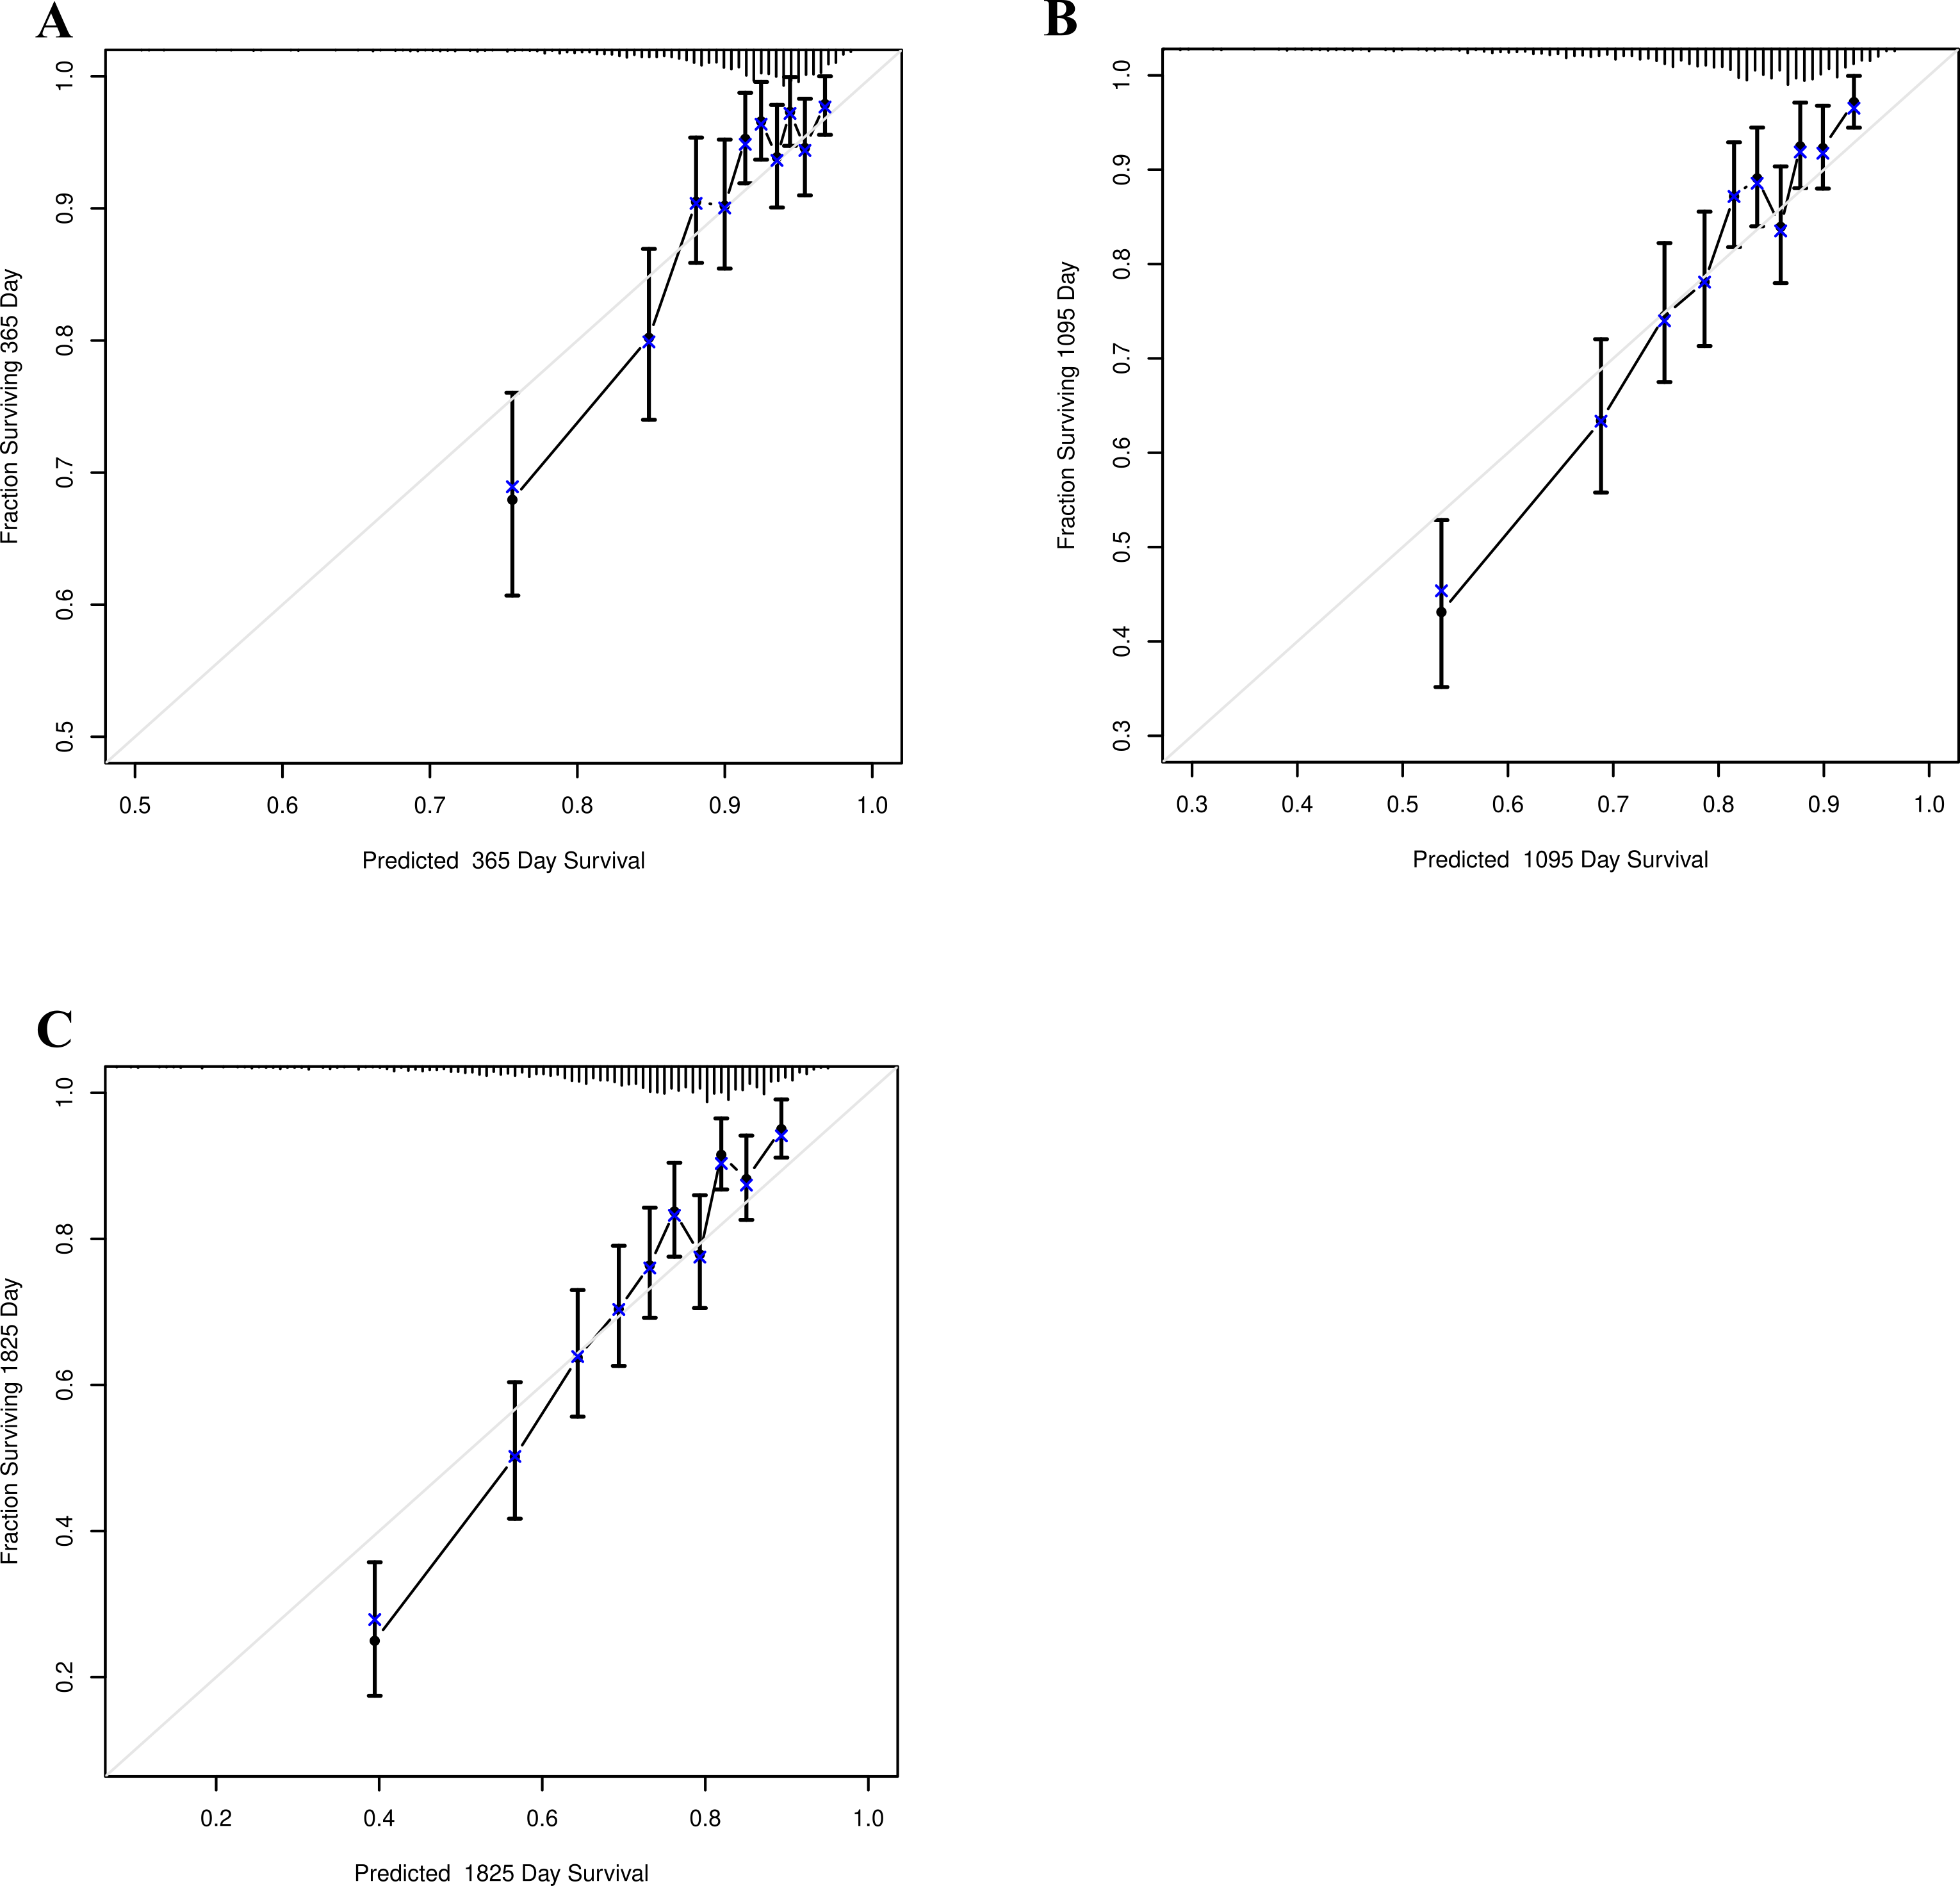
\includegraphics[width=\textwidth]{Chapter3/Figures/Supp_Figure1.png}
  \caption[Prognostic signature calibration curves]{Calibration curves plotting the estimated probabilities (x-axis) vs. the observed BCR events (y-axis) for years 1 (A), 3 (B) and 5 (C), respectively. Estimated probabilities were derived using the derivation dataset.}
  \label{chp4suppfigure1}
\end{figure}

\subsection{Supplementary Files}
\hypertarget{chp4suppfile1}{}

LNCaP miRNA sequencing counts are available online at the following \href{https://github.com/BarryDigby/pca_network/blob/main/mirna/LNCaP/mirna.tsv}{link}.